
%NOTE: to be used with \usepackage{subfiles} in the main file.
%Subfiles go in folders which live with the main file.
%Bibliography and preamble go in the main file.

%%%%%%%%%%%%%%%%%%%%%%%% PREAMBLE %%%%%%%%%%%%%%%%%%%%%%%%
\providecommand{\main}{..}

\documentclass[main]{subfiles} %Each instance of `../' elevates one folder to find the main file

\begin{document}

%%%%%%%%%%%%%%%%%%%%%%% DOCUMENT %%%%%%%%%%%%%%%%%%%%%%%

% \tableofcontents % Can be useful to load a TOC while writing

\doublespacing

\schapter{Results}
\label{sect:results}
\vspace{20pt}

An initial assessment of the discriminant capabilities of the substructure variables studied in this work can be done by looking at the difference in their distributions for signal and background events. The distributions for multiple fat jet variables in the training sample events for both the top signal and the QCD background are shown in figure \ref{fig:top_distributions}.\\

As can be seen from figures \ref{fig:top_distributions}(a) - \ref{fig:top_distributions}(d) the $\tau_N$ variables do not possess a significant discriminant power by themselves due to the lack of separation between the signal and background distributions. This makes a cut based selection based on these variables alone effectively impossible. On the other hand, the distributions of the $\tau_{N+1}/\tau_N$ ratios exhibit a much better separation between background and signal, as depicted in figures \ref{fig:top_distributions}(e) - \ref{fig:top_distributions}(g). Although these ratios are not needed as input variables in the tagging method proposed, their distributions are plotted because they account for the discussion presented in section \ref{sect:substructure} and reinforce the advantages of a multivariate analysis. \\

The statements made above also hold true when the variable distributions for the $W$ signal are taken into account. The variable distributions for the training sample events of the $W$ signal are plotted against those of the QCD background in figure \ref{fig:W_distributions}. However one remark can be made regarding the difference with the top signal $\tau_{N+1}/\tau_N$ distributions. As can be seen in figures \ref{fig:W_distributions}(e) - \ref{fig:W_distributions}(g), for the $W$ signal the ratio $\tau_2/\tau_1$ exhibits the best separation between the signal and background distributions. That is not the case for the 

\begin{figure}[H]
     \centering
     \begin{subfigure}[h]{0.49\textwidth}
         \centering
         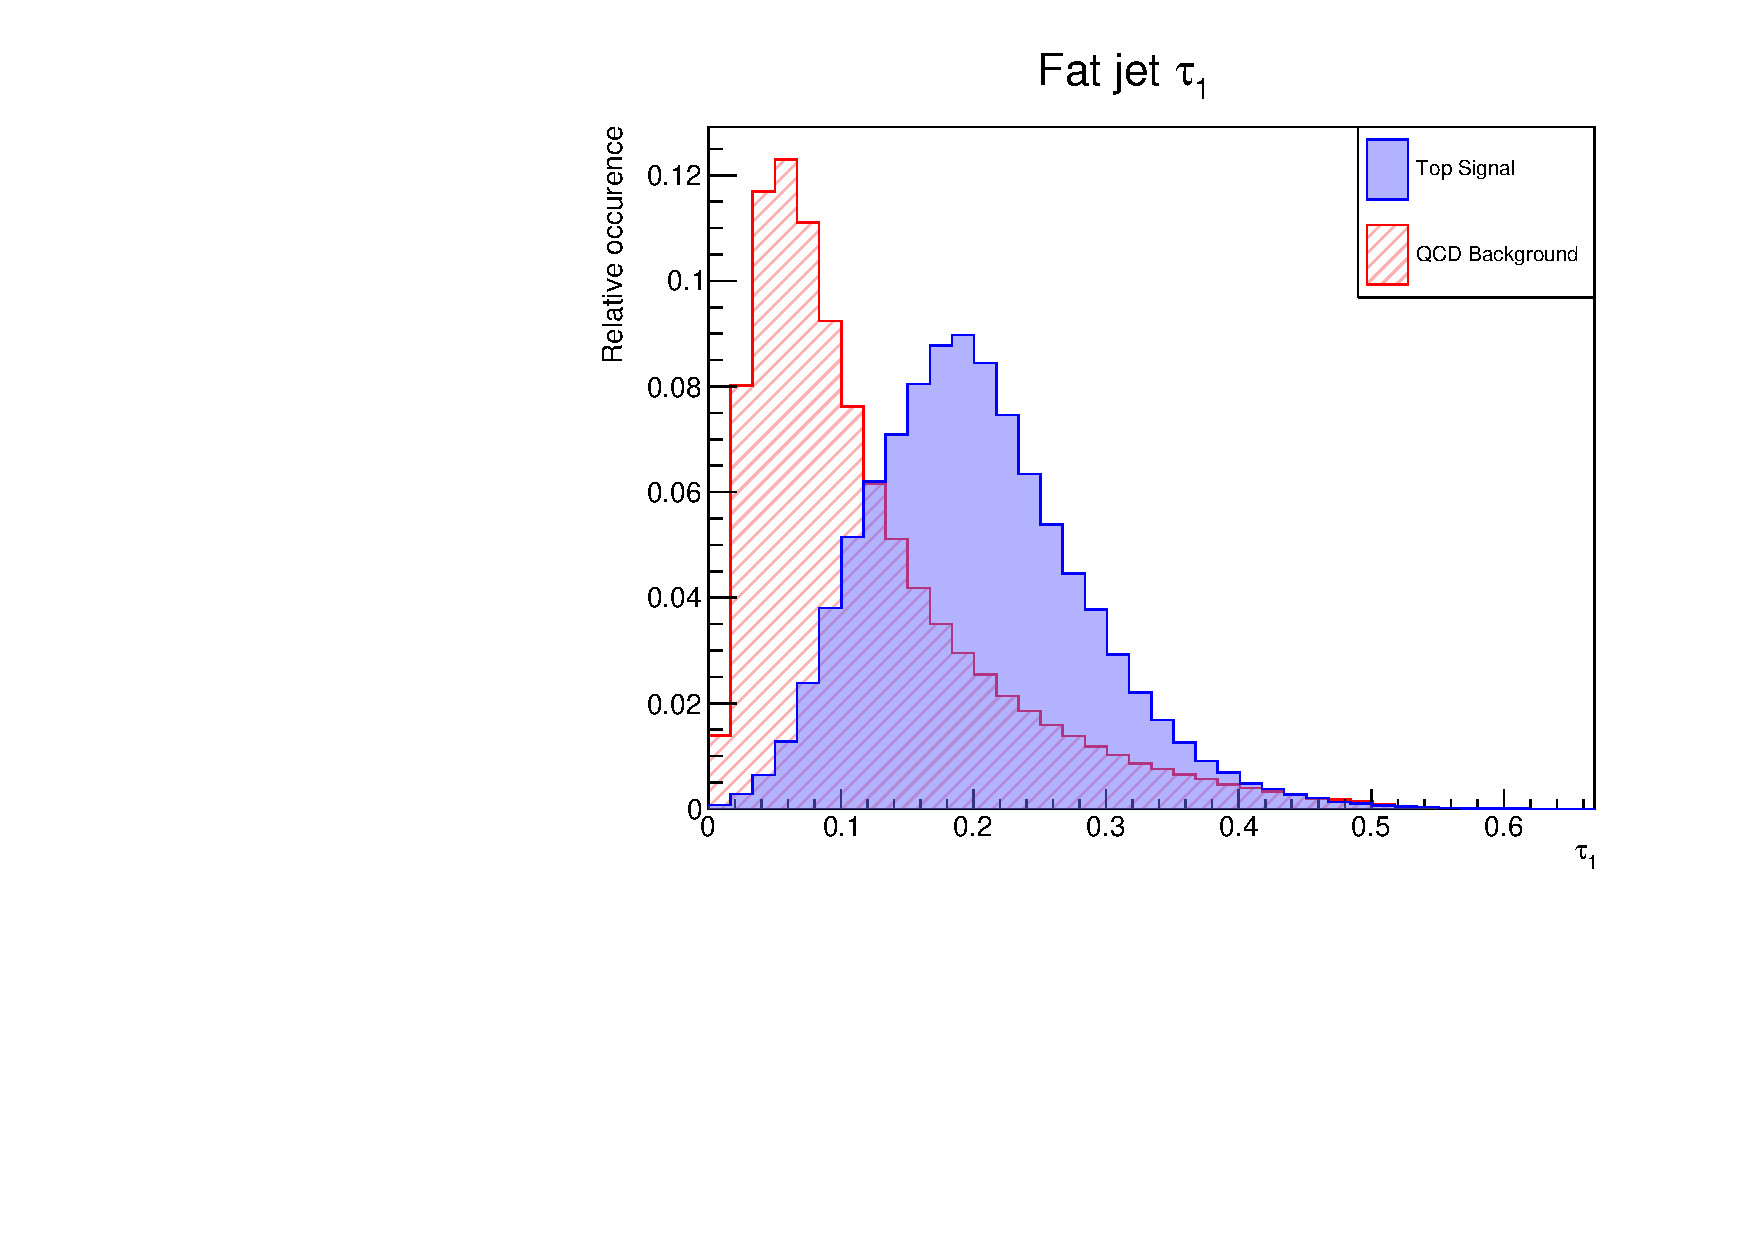
\includegraphics[width=0.8\textwidth]{../Figures/Results/top_distributions/top_tau1_distribution.pdf}
          \caption{}
         \label{fig:top_distribution_tau1}
     \end{subfigure}
     \begin{subfigure}[h]{0.49\textwidth}
         \centering
         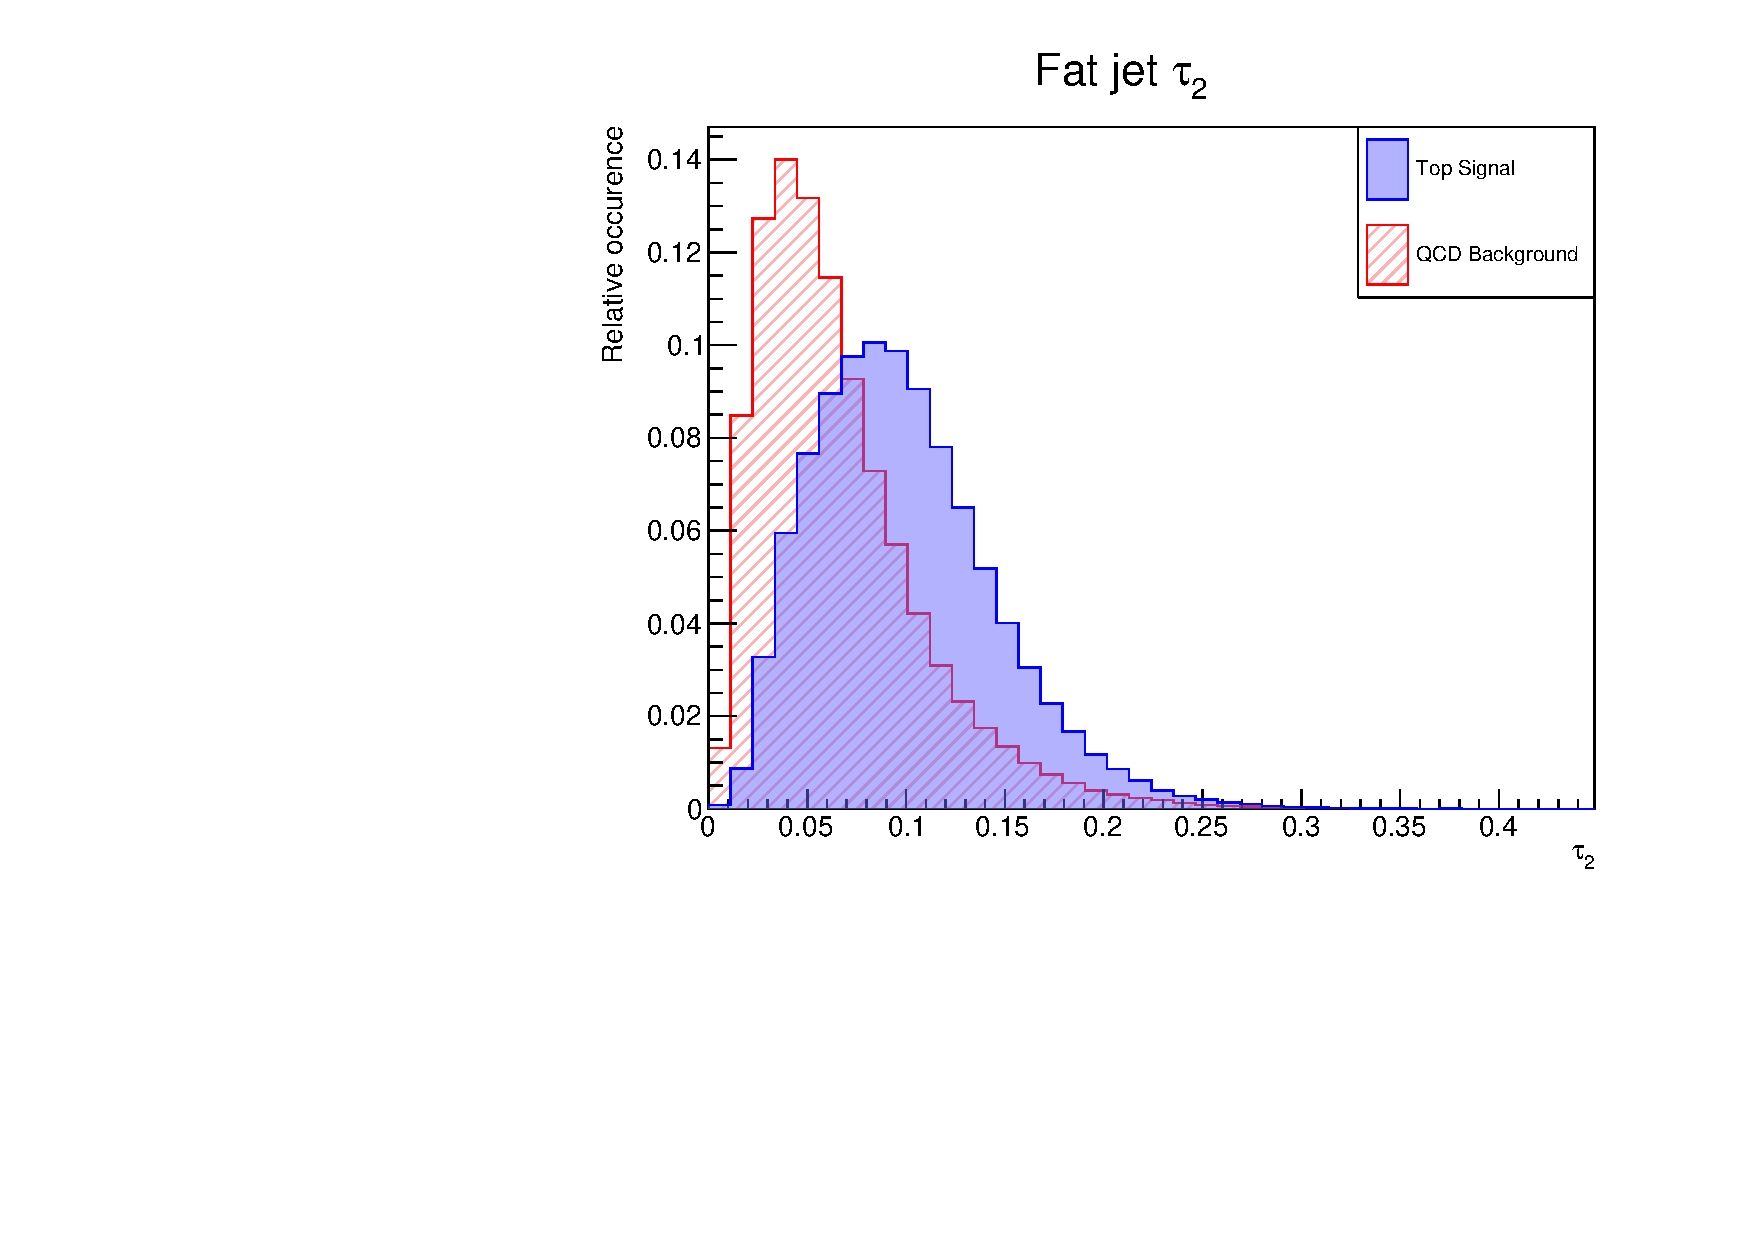
\includegraphics[width=0.8\textwidth]{../Figures/Results/top_distributions/top_tau2_distribution.pdf}
          \caption{}
         \label{fig:top_distribution_tau2}
     \end{subfigure}
     \par\bigskip
     \begin{subfigure}[h]{0.49\textwidth}
         \centering
         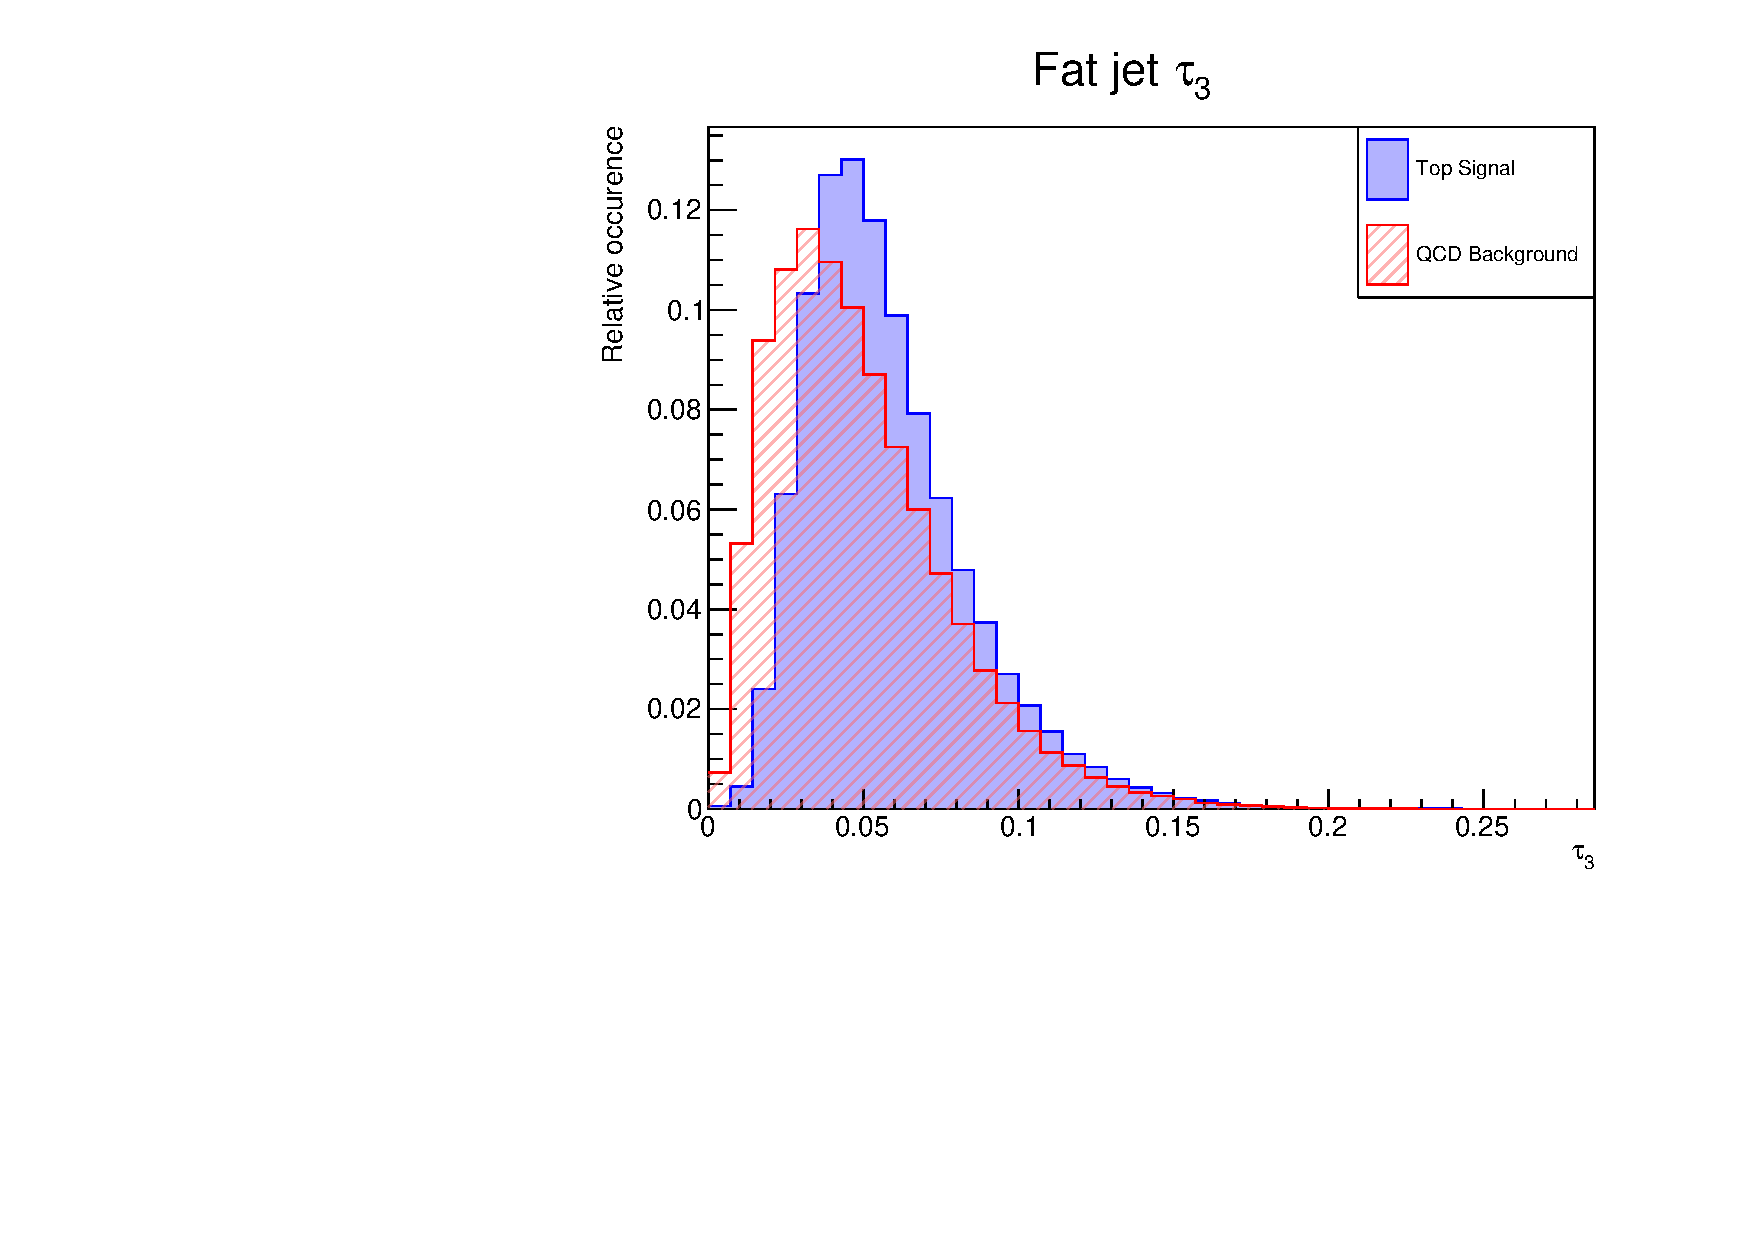
\includegraphics[width=0.8\textwidth]{../Figures/Results/top_distributions/top_tau3_distribution.pdf}
          \caption{}
         \label{fig:top_distribution_tau3}
     \end{subfigure}
     \begin{subfigure}[h]{0.49\textwidth}
         \centering
         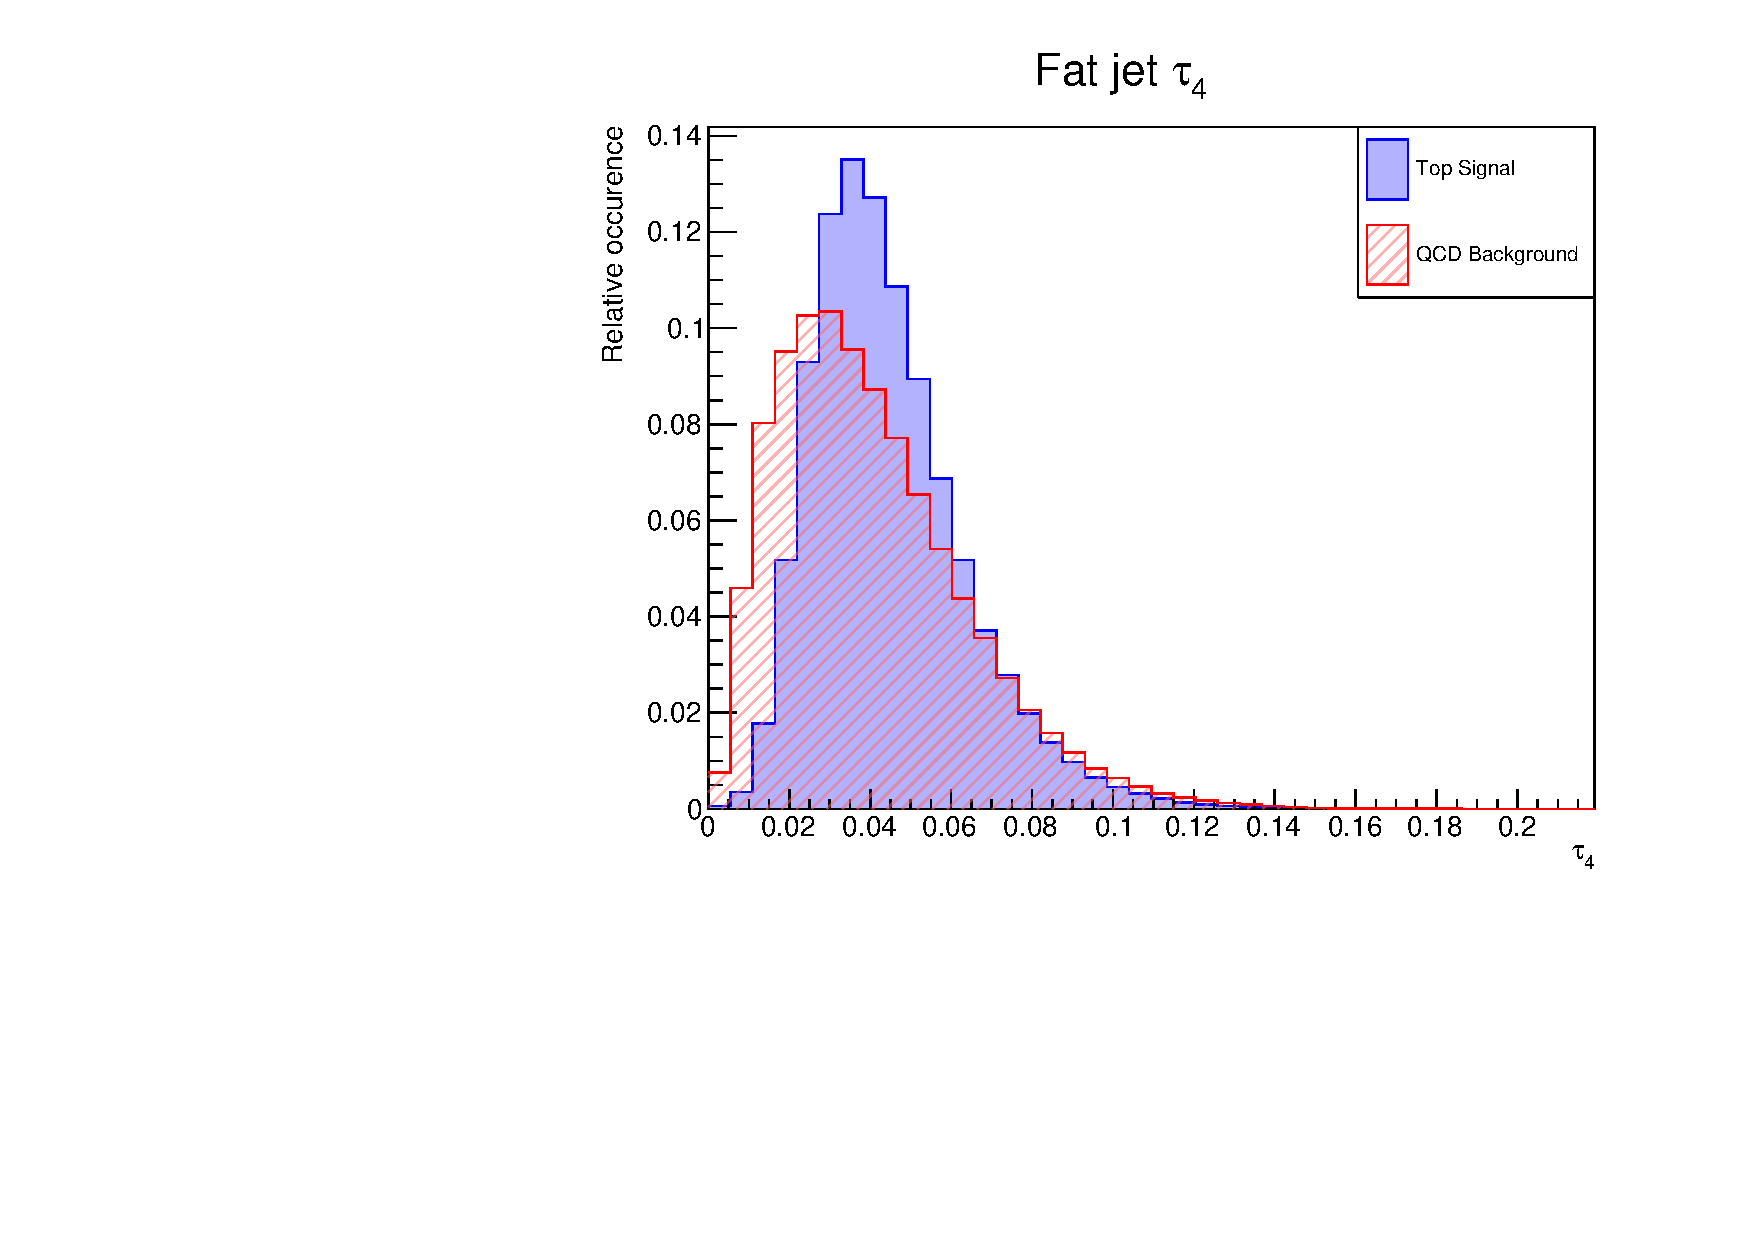
\includegraphics[width=0.8\textwidth]{../Figures/Results/top_distributions/top_tau4_distribution.pdf}
          \caption{}
         \label{fig:top_distribution_tau4}
     \end{subfigure}
     \par\bigskip
     \begin{subfigure}[h]{0.49\textwidth}
         \centering
         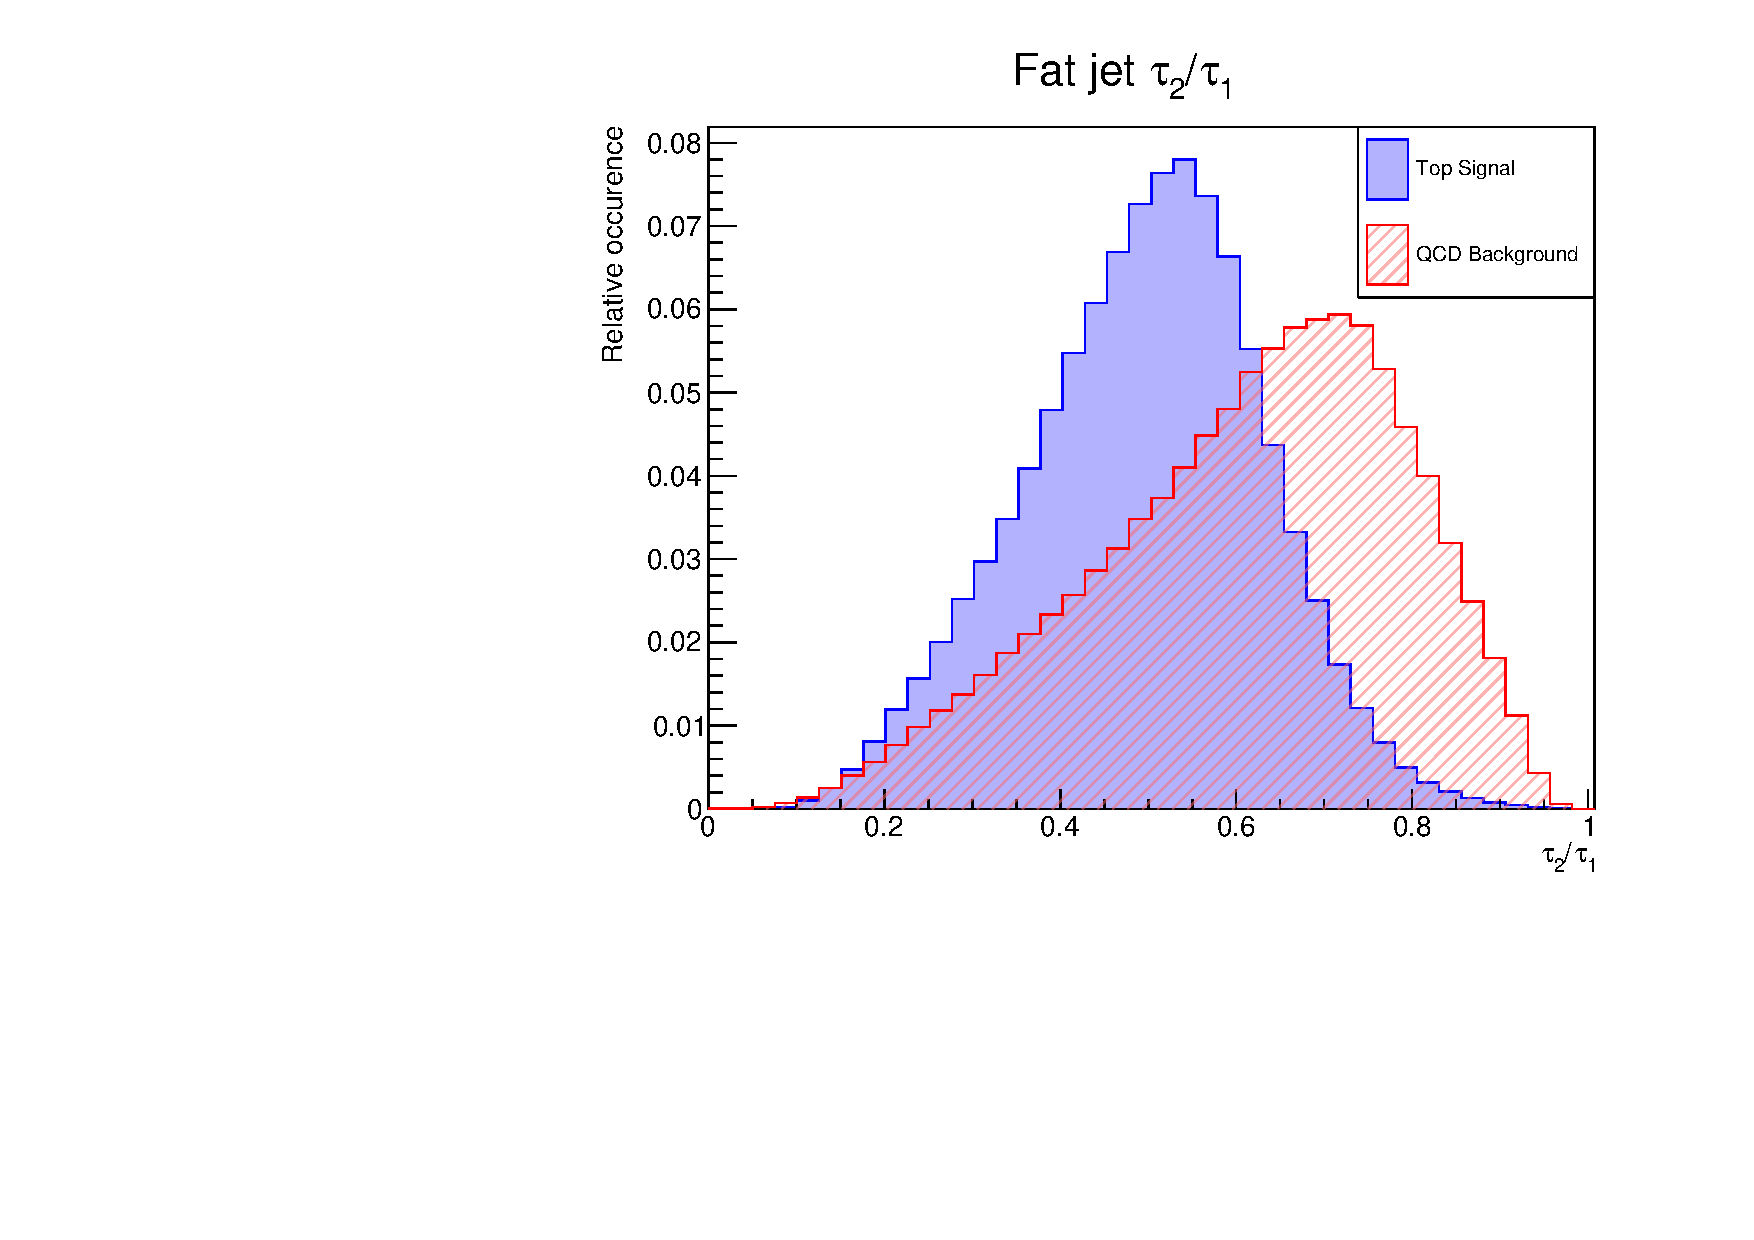
\includegraphics[width=0.8\textwidth]{../Figures/Results/top_distributions/top_tau21_distribution.pdf}
          \caption{}
         \label{fig:top_distribution_tau21}
     \end{subfigure}
     \begin{subfigure}[h]{0.49\textwidth}
         \centering
         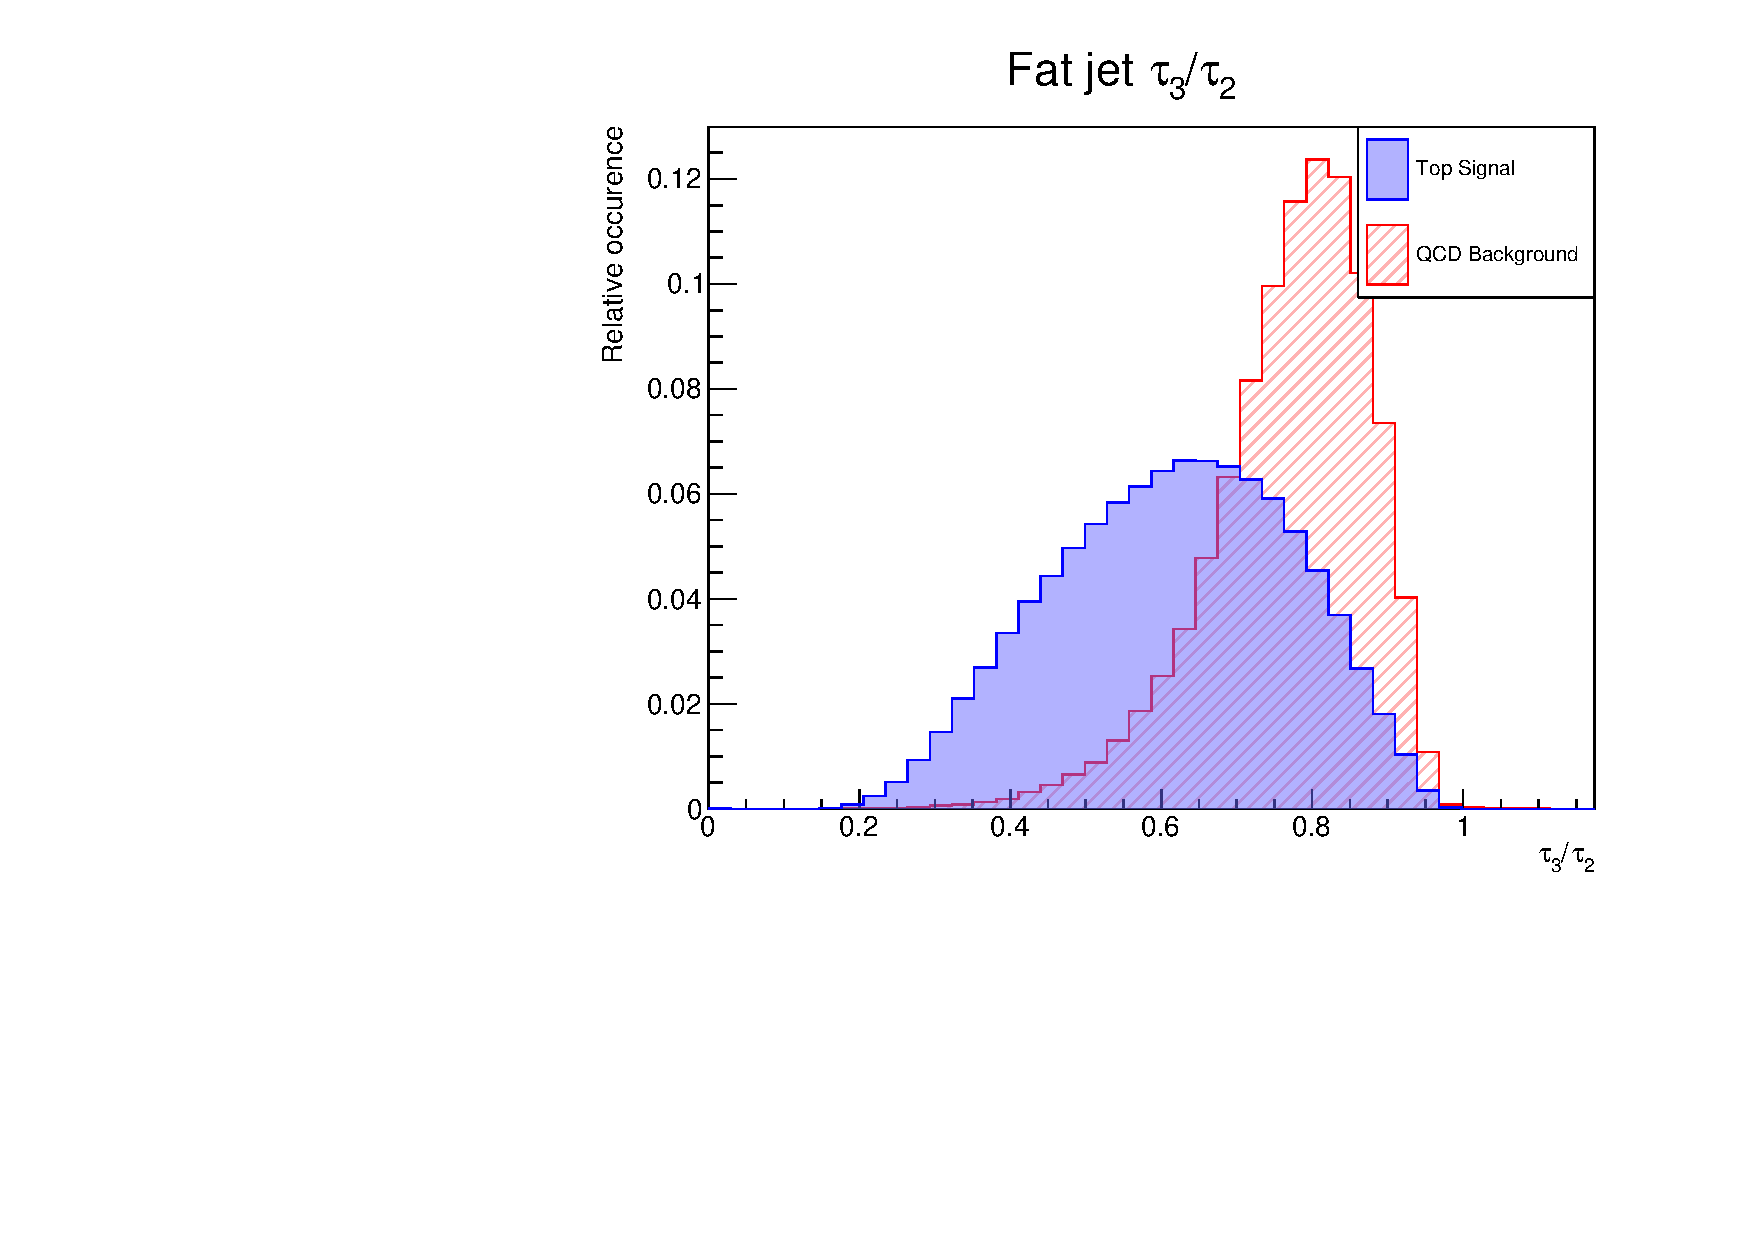
\includegraphics[width=0.8\textwidth]{../Figures/Results/top_distributions/top_tau32_distribution.pdf}
          \caption{}
         \label{fig:top_distribution_tau32}
     \end{subfigure}
     \par\bigskip 
     \begin{subfigure}[h]{0.49\textwidth}
         \centering
         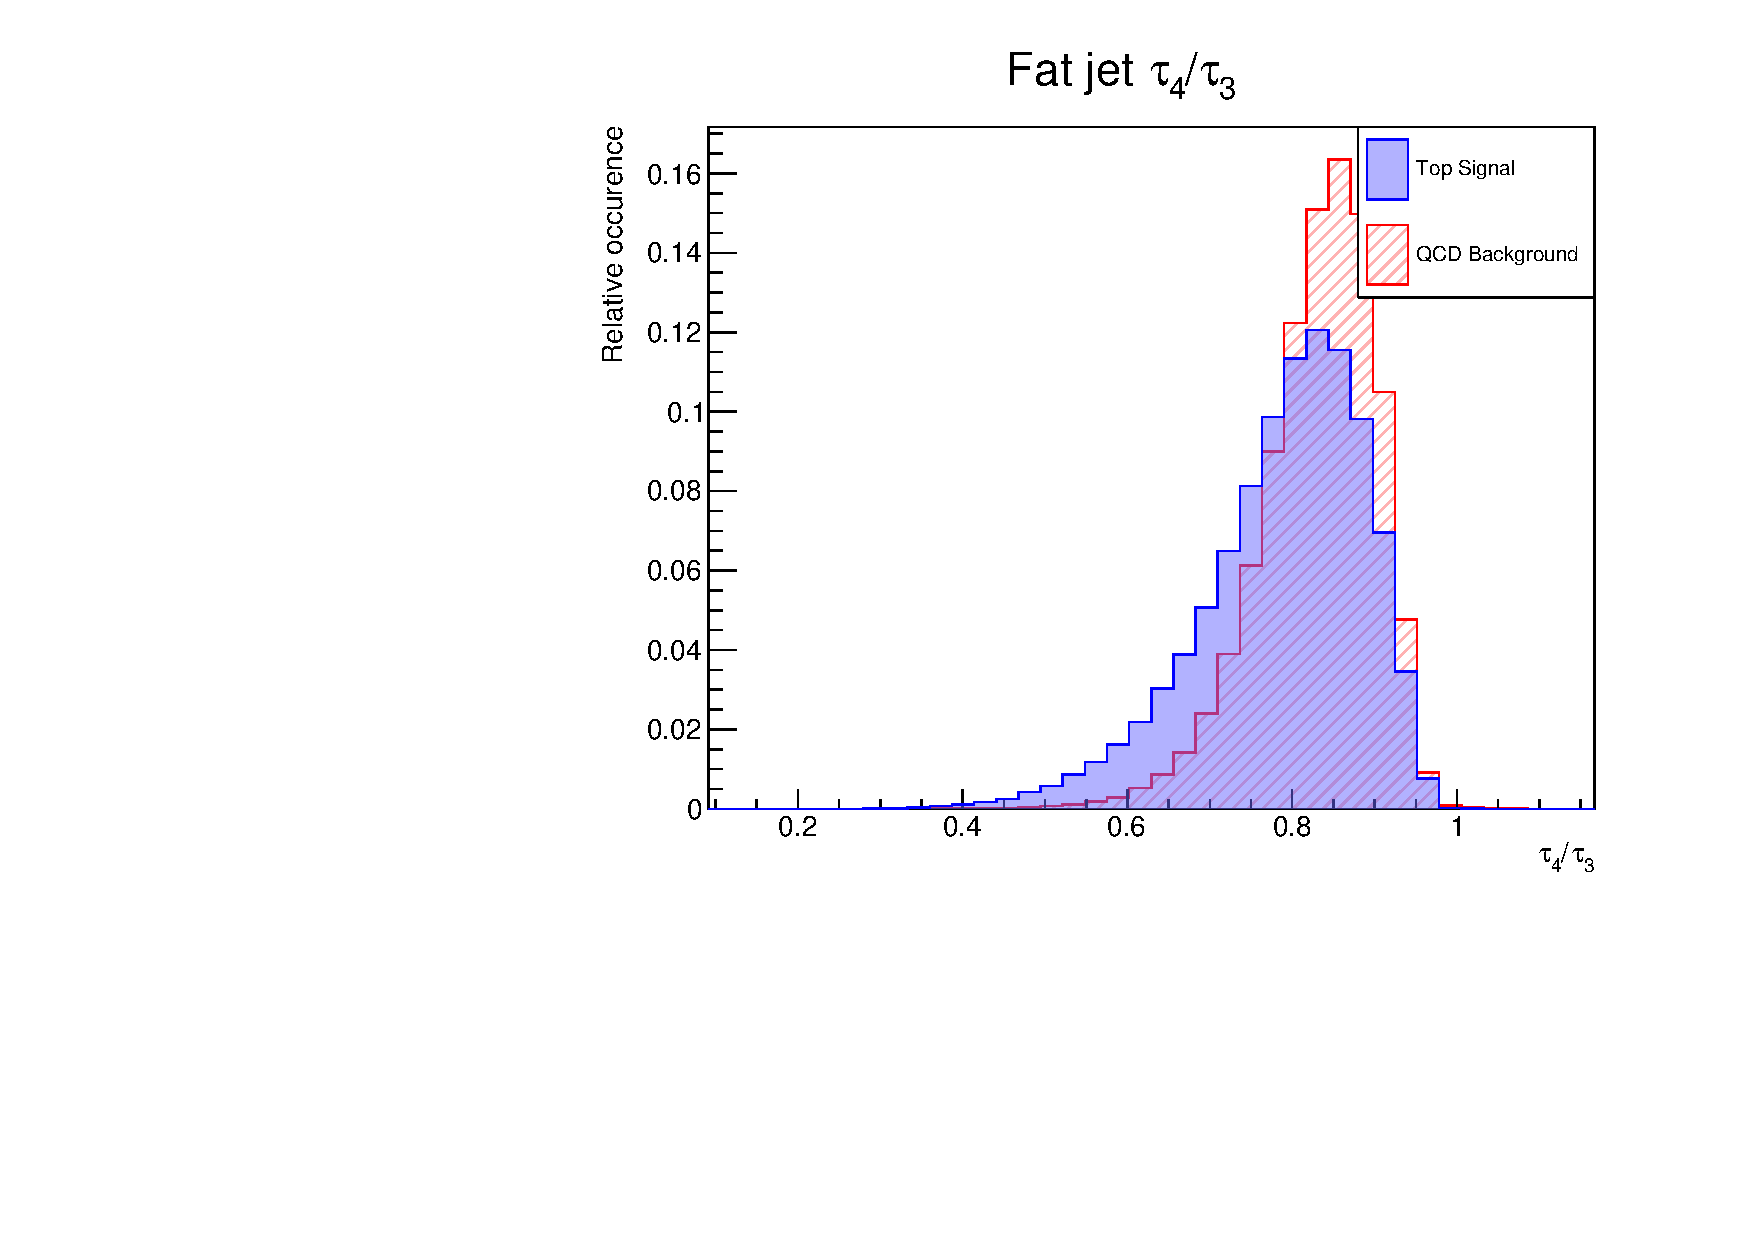
\includegraphics[width=0.8\textwidth]{../Figures/Results/top_distributions/top_tau43_distribution.pdf}
          \caption{}
         \label{fig:top_distribution_tau43}
     \end{subfigure}
     \begin{subfigure}[h]{0.49\textwidth}
         \centering
         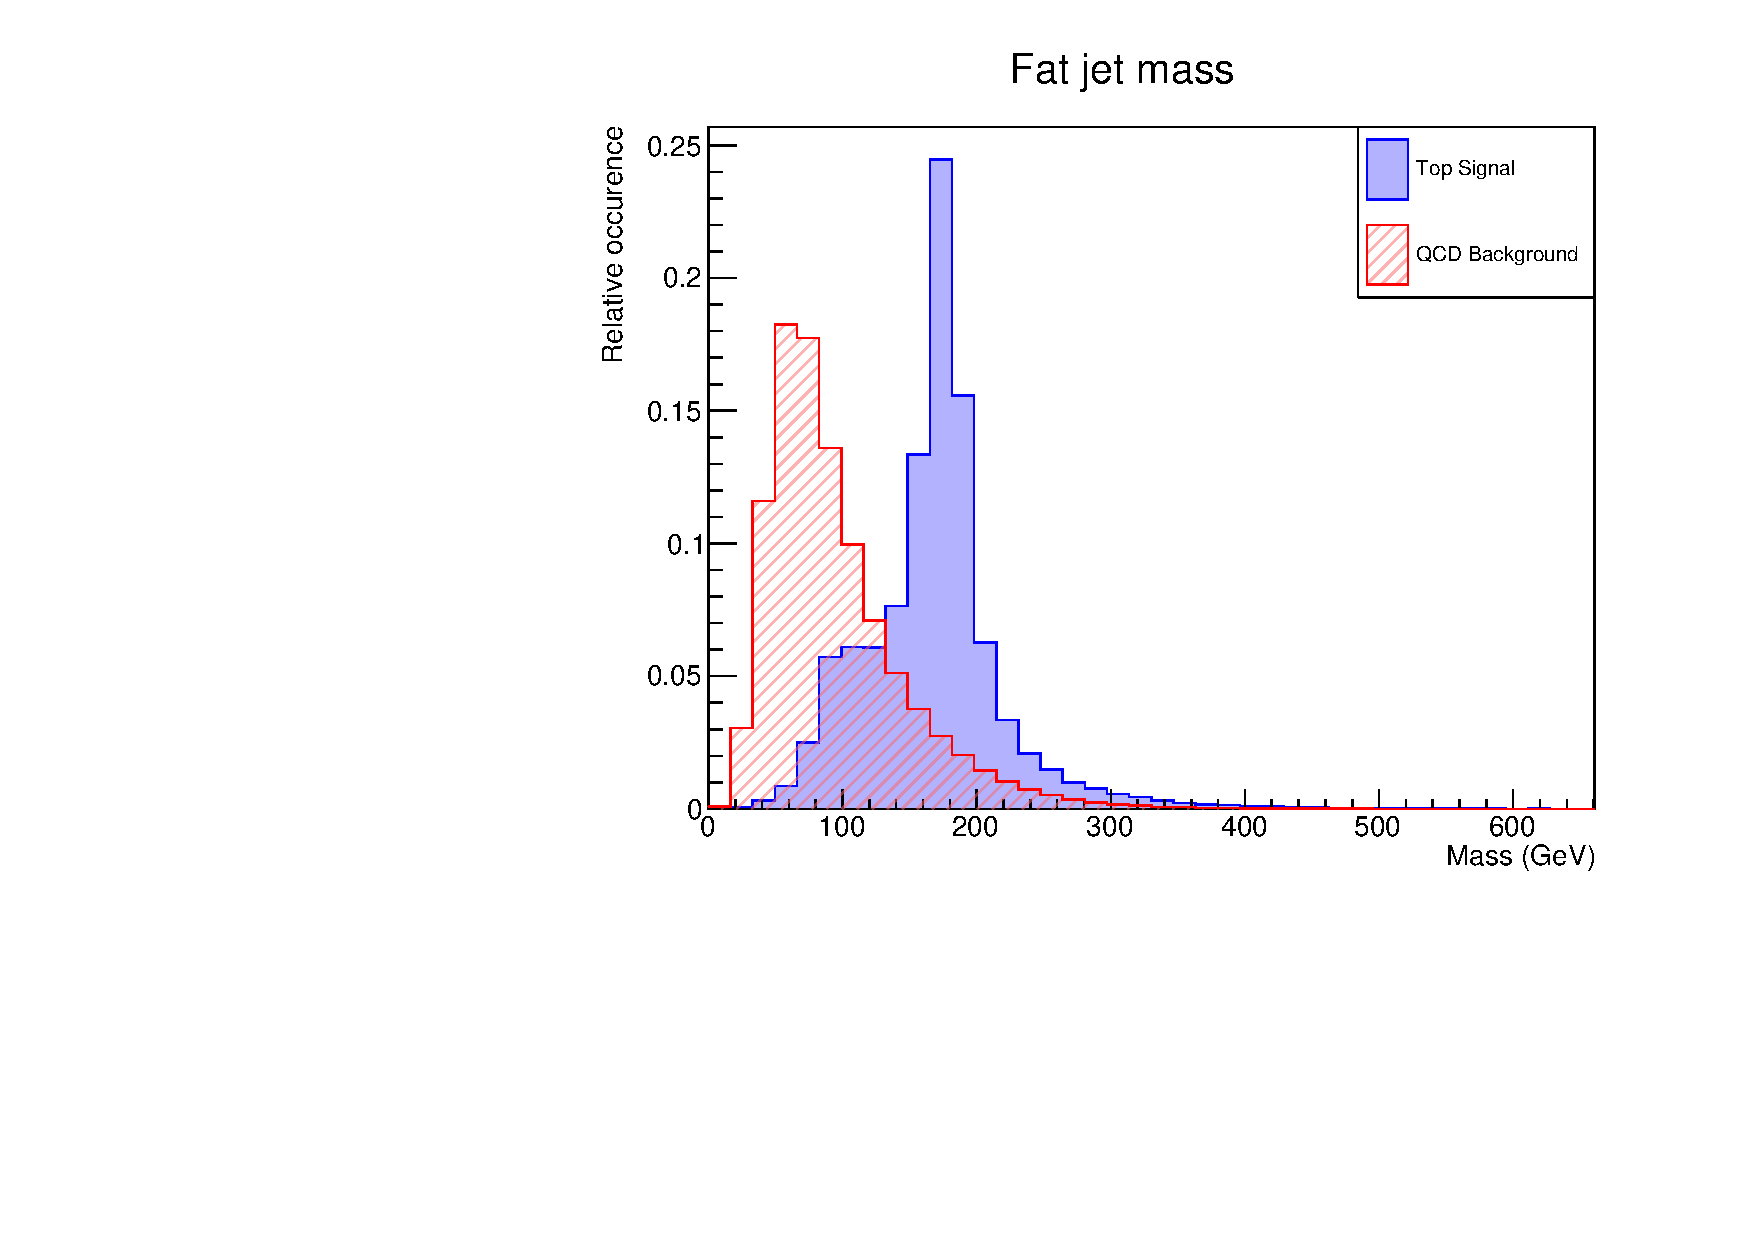
\includegraphics[width=0.8\textwidth]{../Figures/Results/top_distributions/top_mass_distribution.pdf}
          \caption{}
         \label{fig:top_distribution_mass}
     \end{subfigure}
     \caption{Distribution of (a)\;-\;(d) $\tau_N$, (e)\;-\;(g) $\tau_{N+1}/\tau_N$ ratios and (h) mass for the top and QCD fat jets in the training sample events.}
        \label{fig:top_distributions}
\end{figure}


\begin{figure}[H]
     \centering
     \begin{subfigure}[h]{0.49\textwidth}
         \centering
         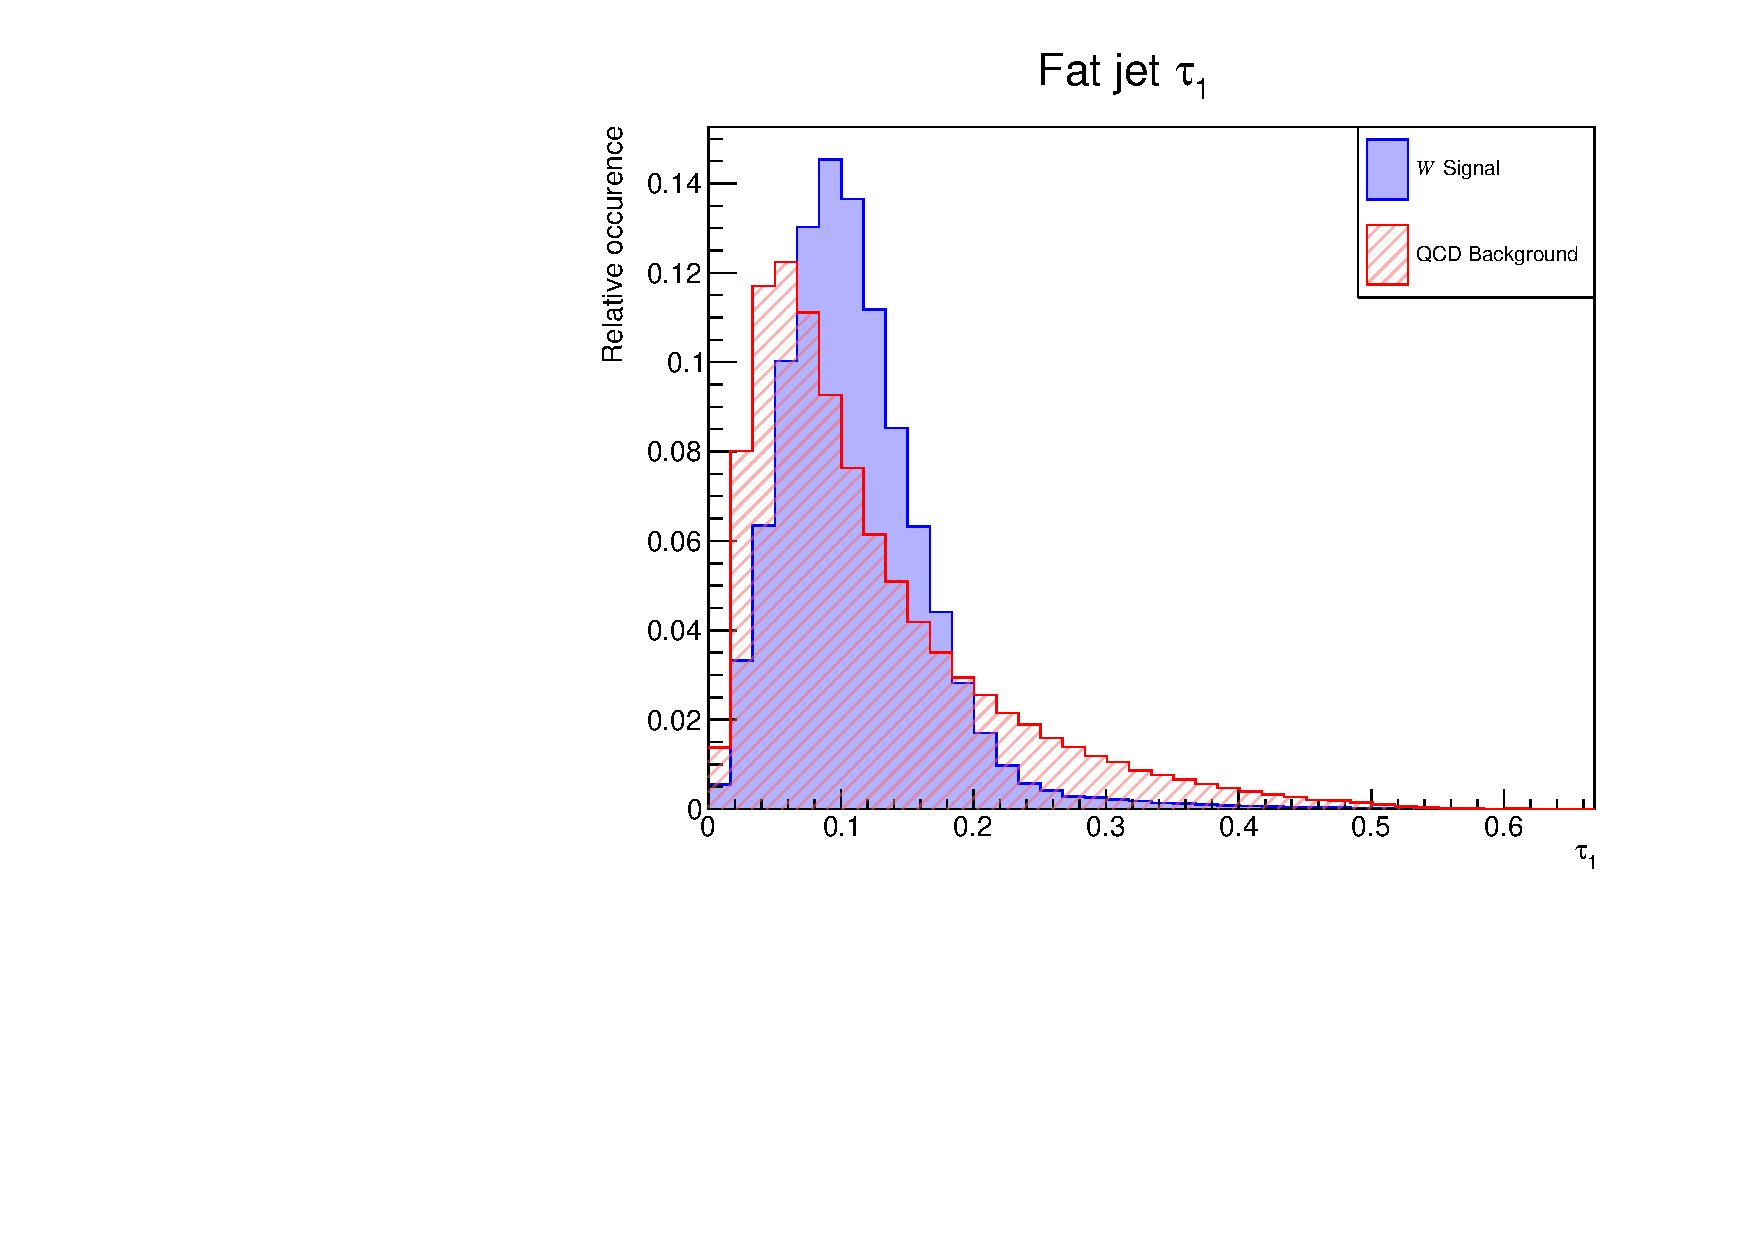
\includegraphics[width=0.8\textwidth]{../Figures/Results/W_distributions/W_tau1_distribution.pdf}
          \caption{}
         \label{fig:W_distribution_tau1}
     \end{subfigure}
     \begin{subfigure}[h]{0.49\textwidth}
         \centering
         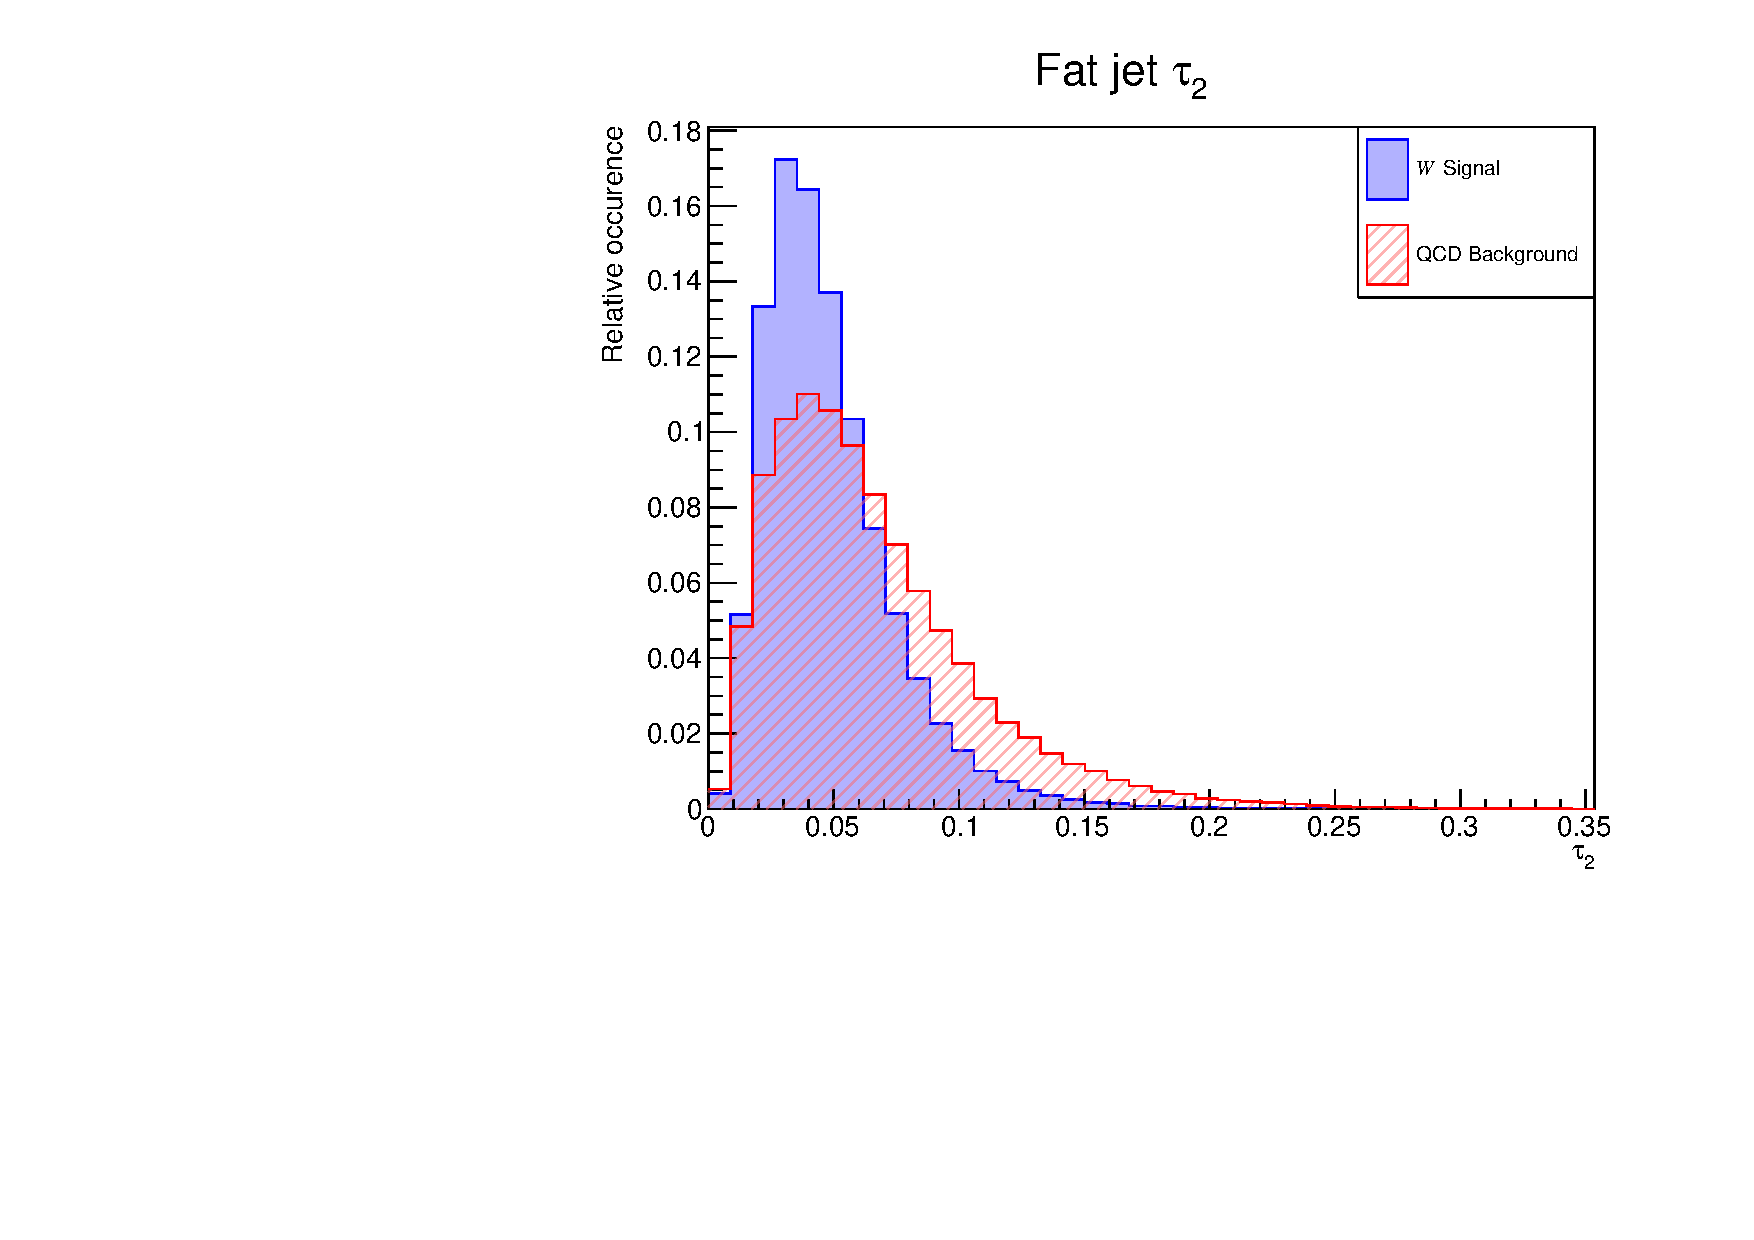
\includegraphics[width=0.8\textwidth]{../Figures/Results/W_distributions/W_tau2_distribution.pdf}
          \caption{}
         \label{fig:W_distribution_tau2}
     \end{subfigure}
     \par\bigskip
     \begin{subfigure}[h]{0.49\textwidth}
         \centering
         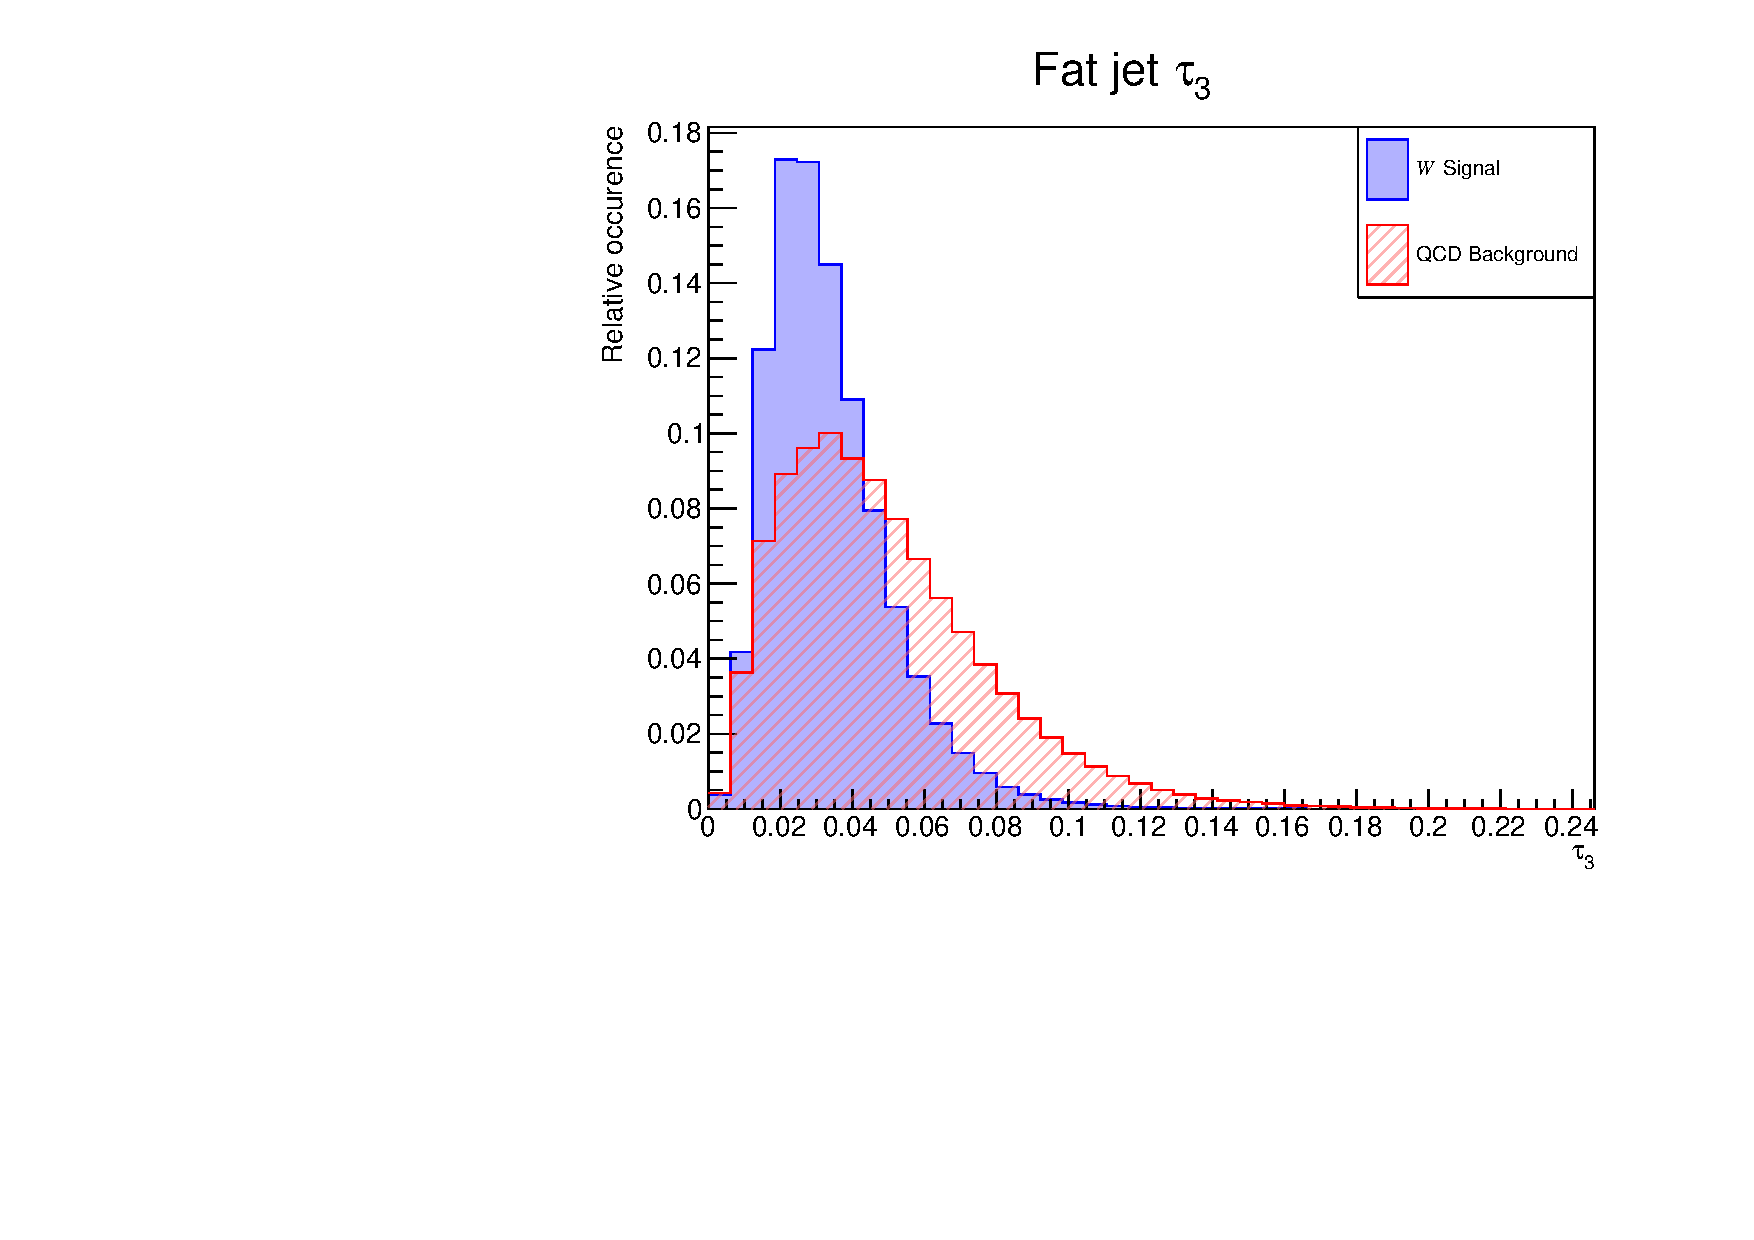
\includegraphics[width=0.8\textwidth]{../Figures/Results/W_distributions/W_tau3_distribution.pdf}
          \caption{}
         \label{fig:W_distribution_tau3}
     \end{subfigure}
     \begin{subfigure}[h]{0.49\textwidth}
         \centering
         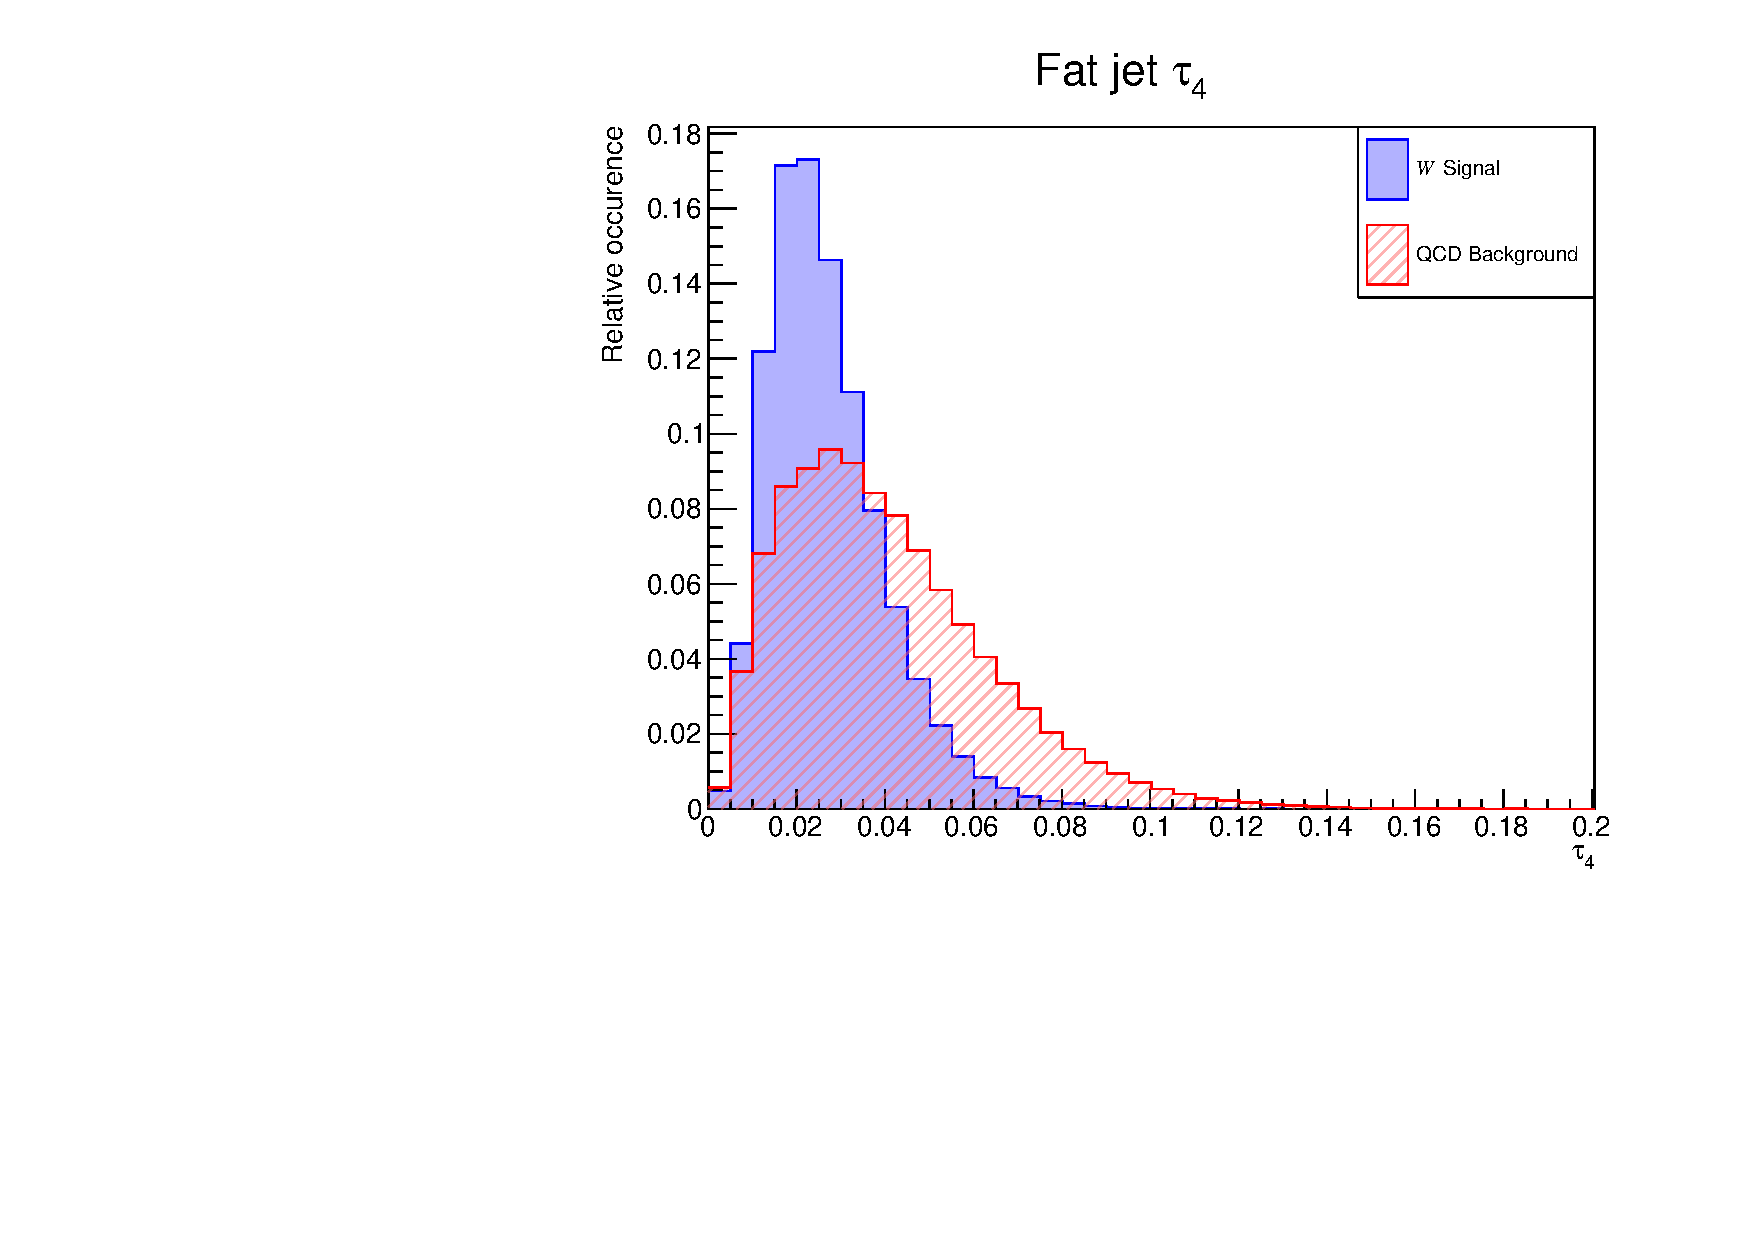
\includegraphics[width=0.8\textwidth]{../Figures/Results/W_distributions/W_tau4_distribution.pdf}
          \caption{}
         \label{fig:W_distribution_tau4}
     \end{subfigure}
     \par\bigskip
     \begin{subfigure}[h]{0.49\textwidth}
         \centering
         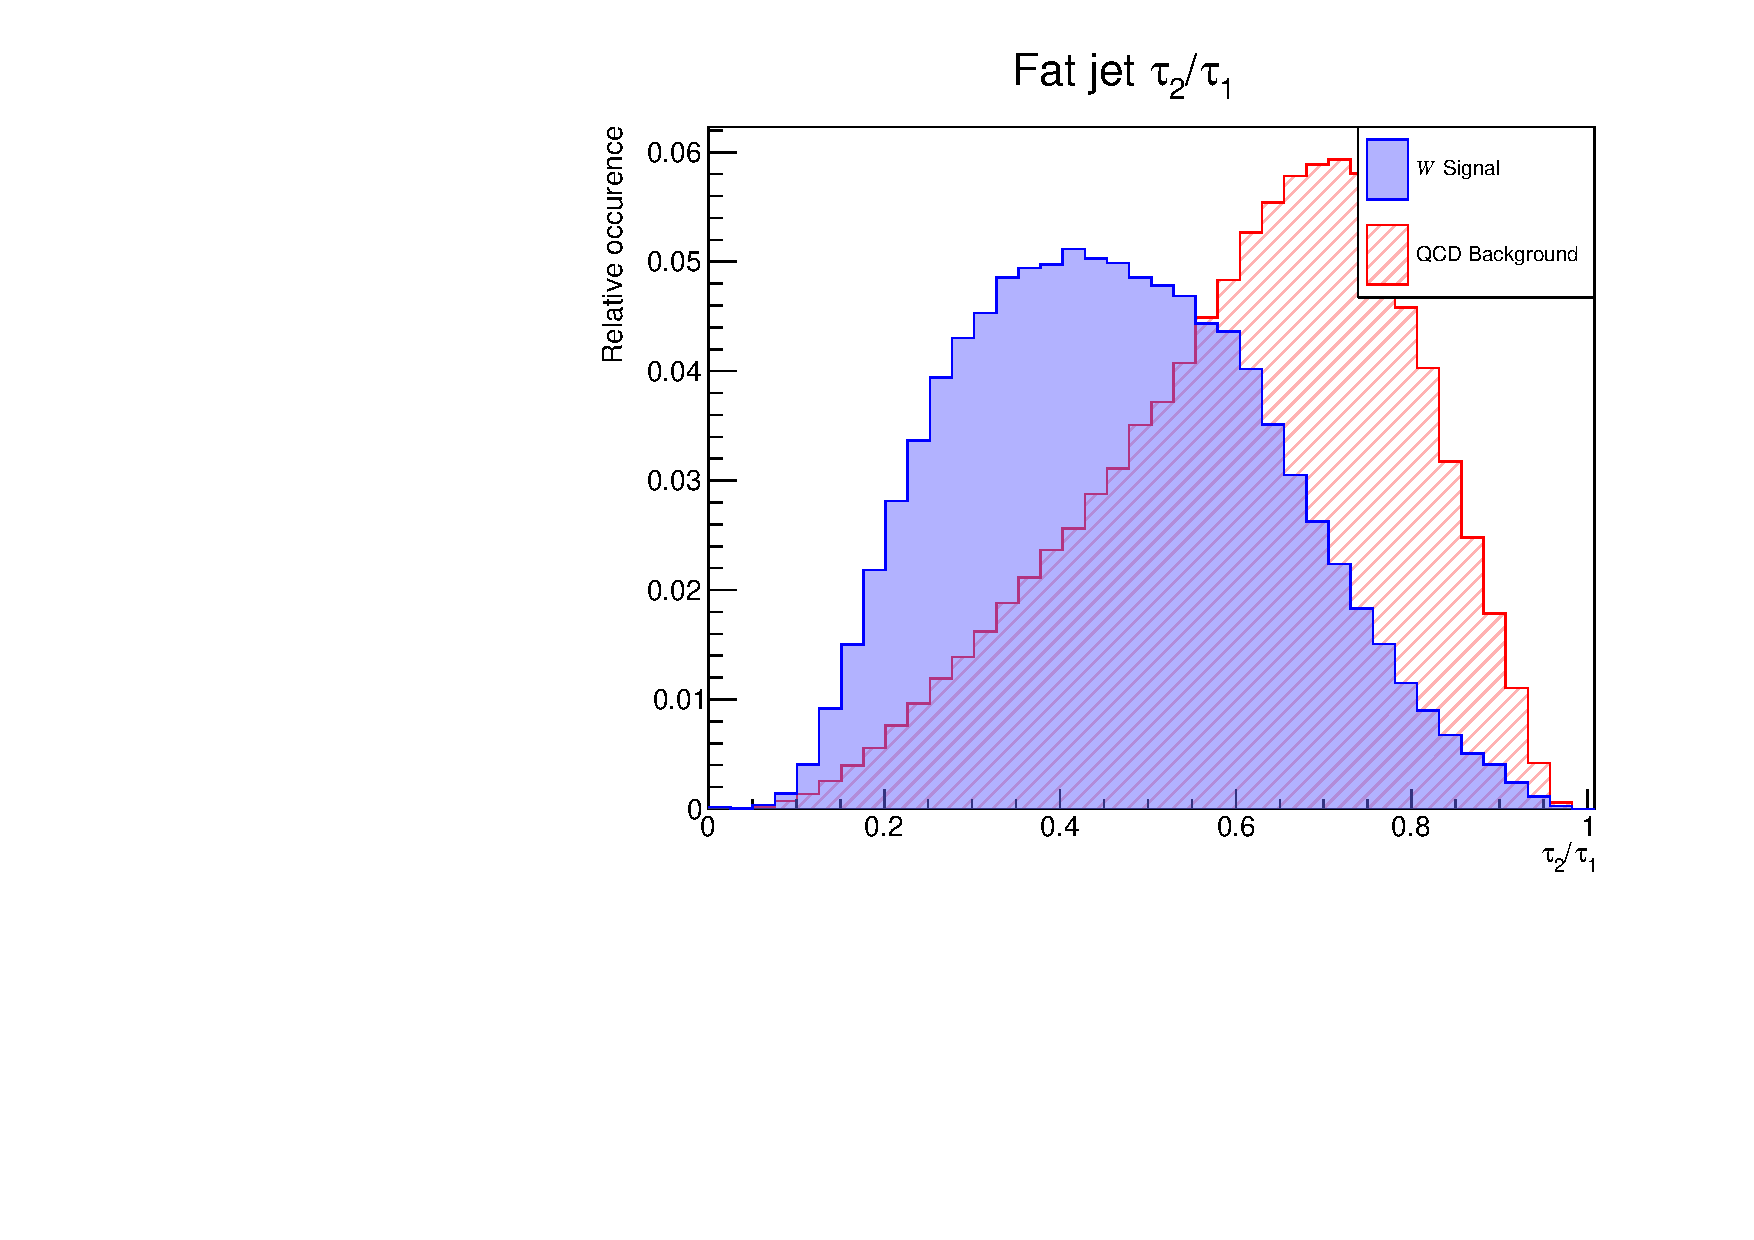
\includegraphics[width=0.8\textwidth]{../Figures/Results/W_distributions/W_tau21_distribution.pdf}
          \caption{}
         \label{fig:W_distribution_tau21}
     \end{subfigure}
     \begin{subfigure}[h]{0.49\textwidth}
         \centering
         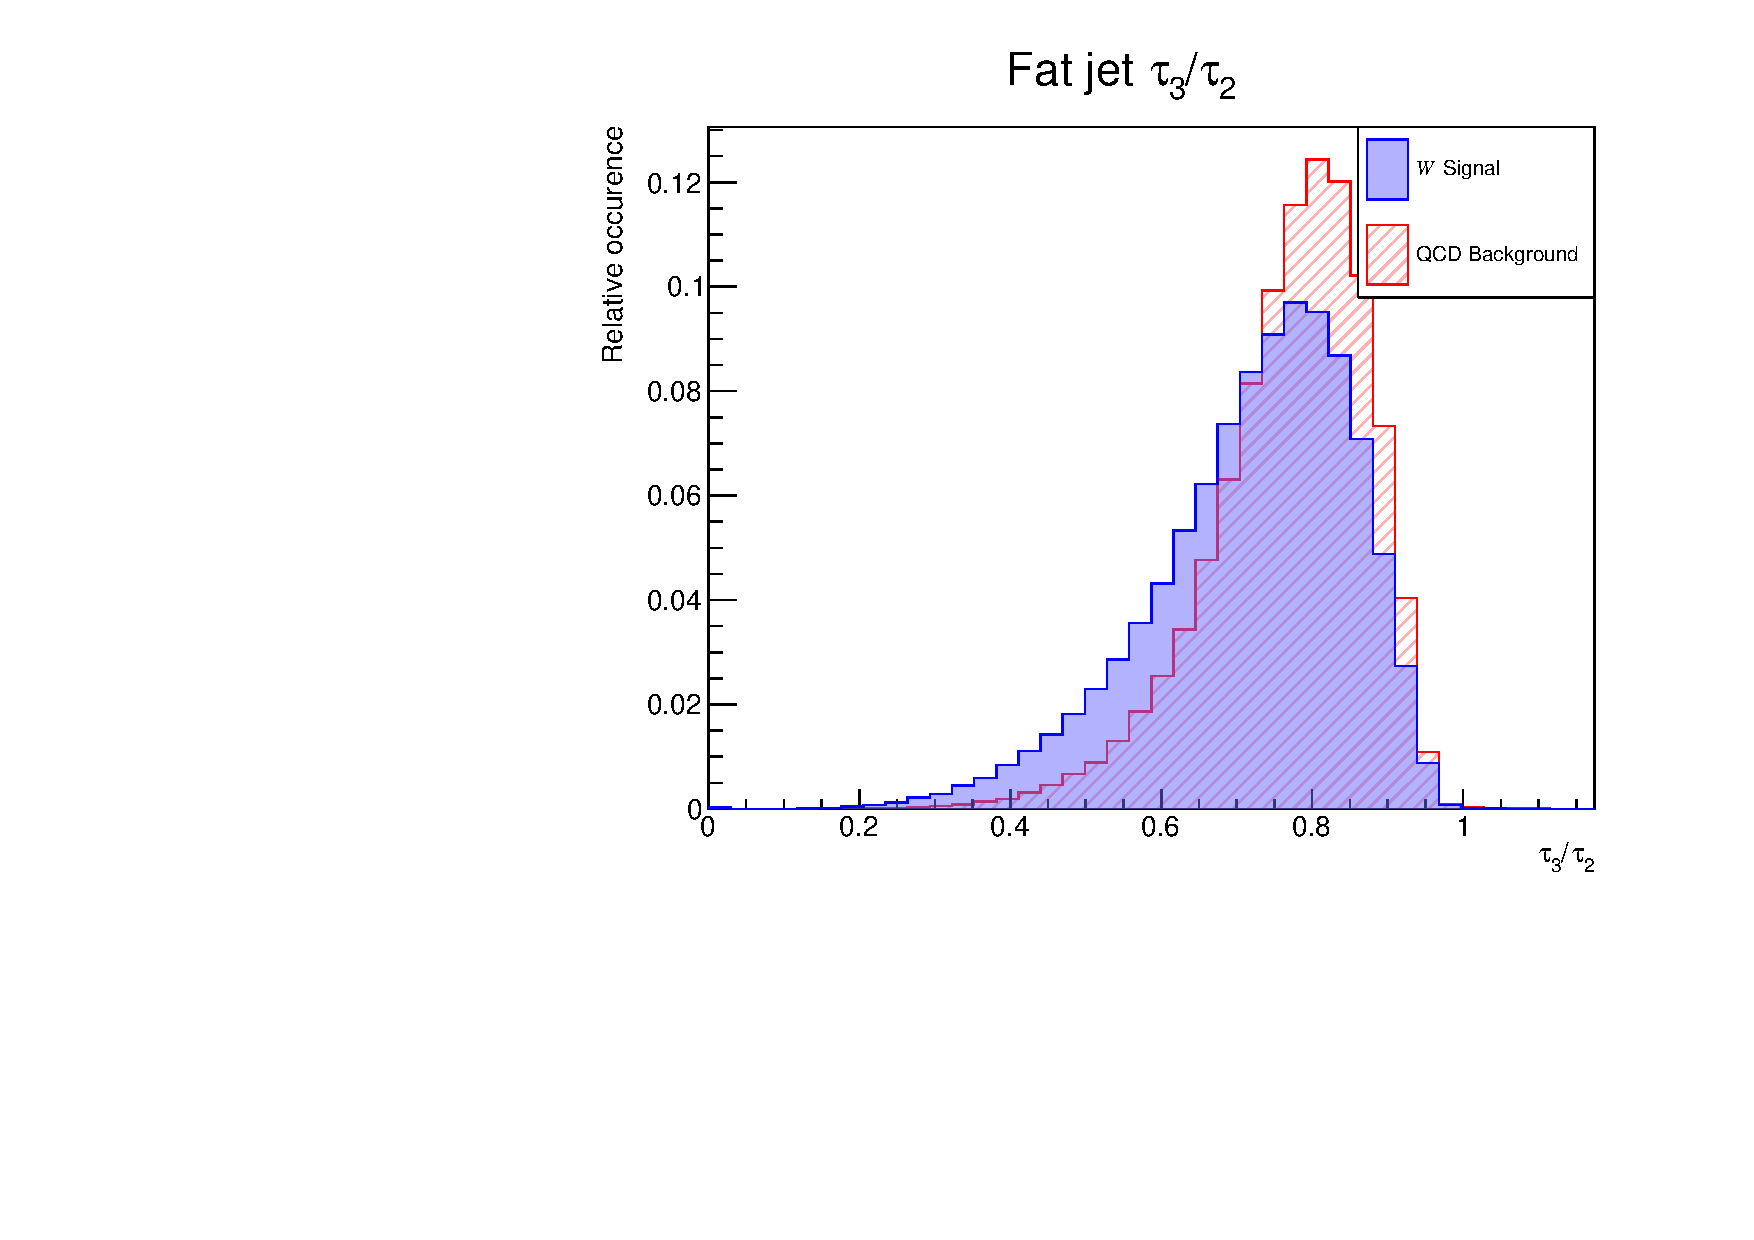
\includegraphics[width=0.8\textwidth]{../Figures/Results/W_distributions/W_tau32_distribution.pdf}
          \caption{}
         \label{fig:W_distribution_tau32}
     \end{subfigure}
     \par\bigskip 
     \begin{subfigure}[h]{0.49\textwidth}
         \centering
         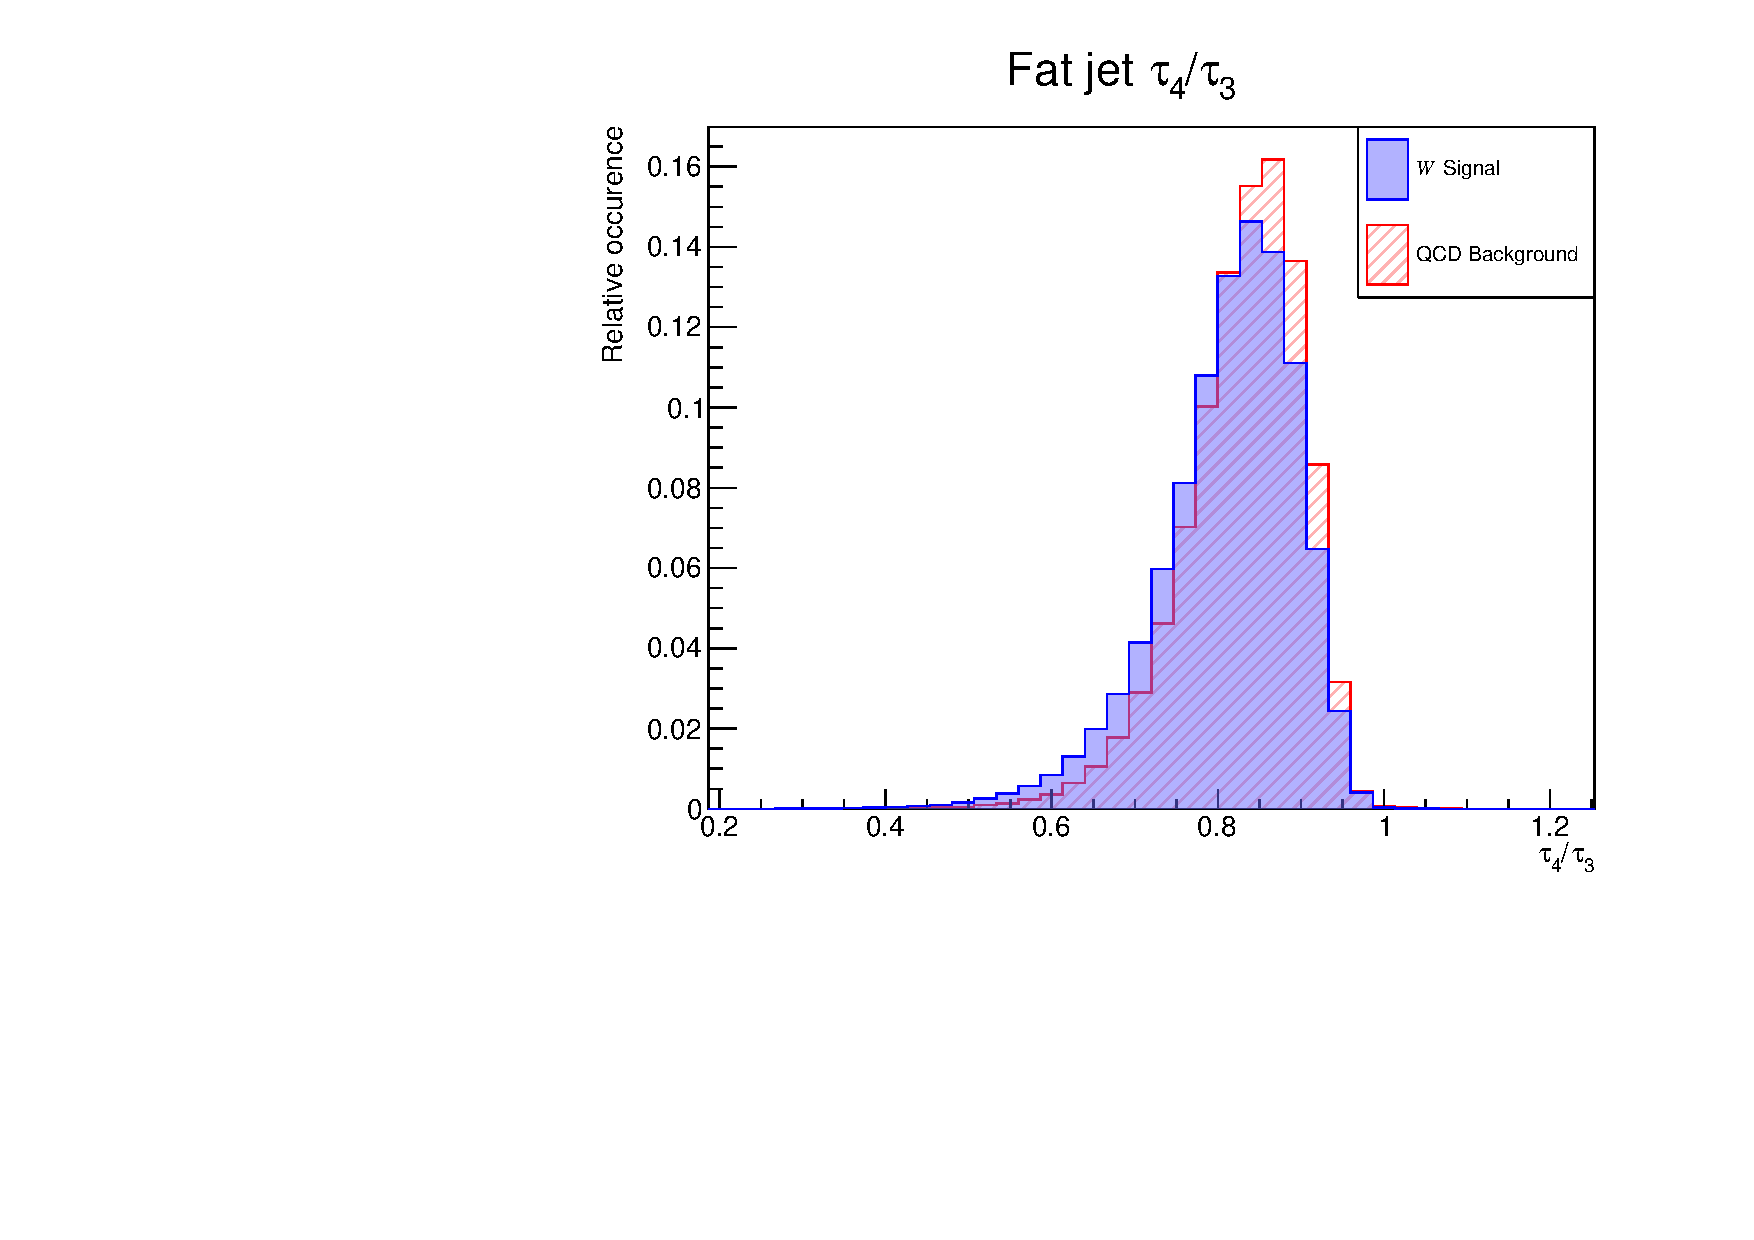
\includegraphics[width=0.8\textwidth]{../Figures/Results/W_distributions/W_tau43_distribution.pdf}
          \caption{}
         \label{fig:W_distribution_tau43}
     \end{subfigure}
     \begin{subfigure}[h]{0.49\textwidth}
         \centering
         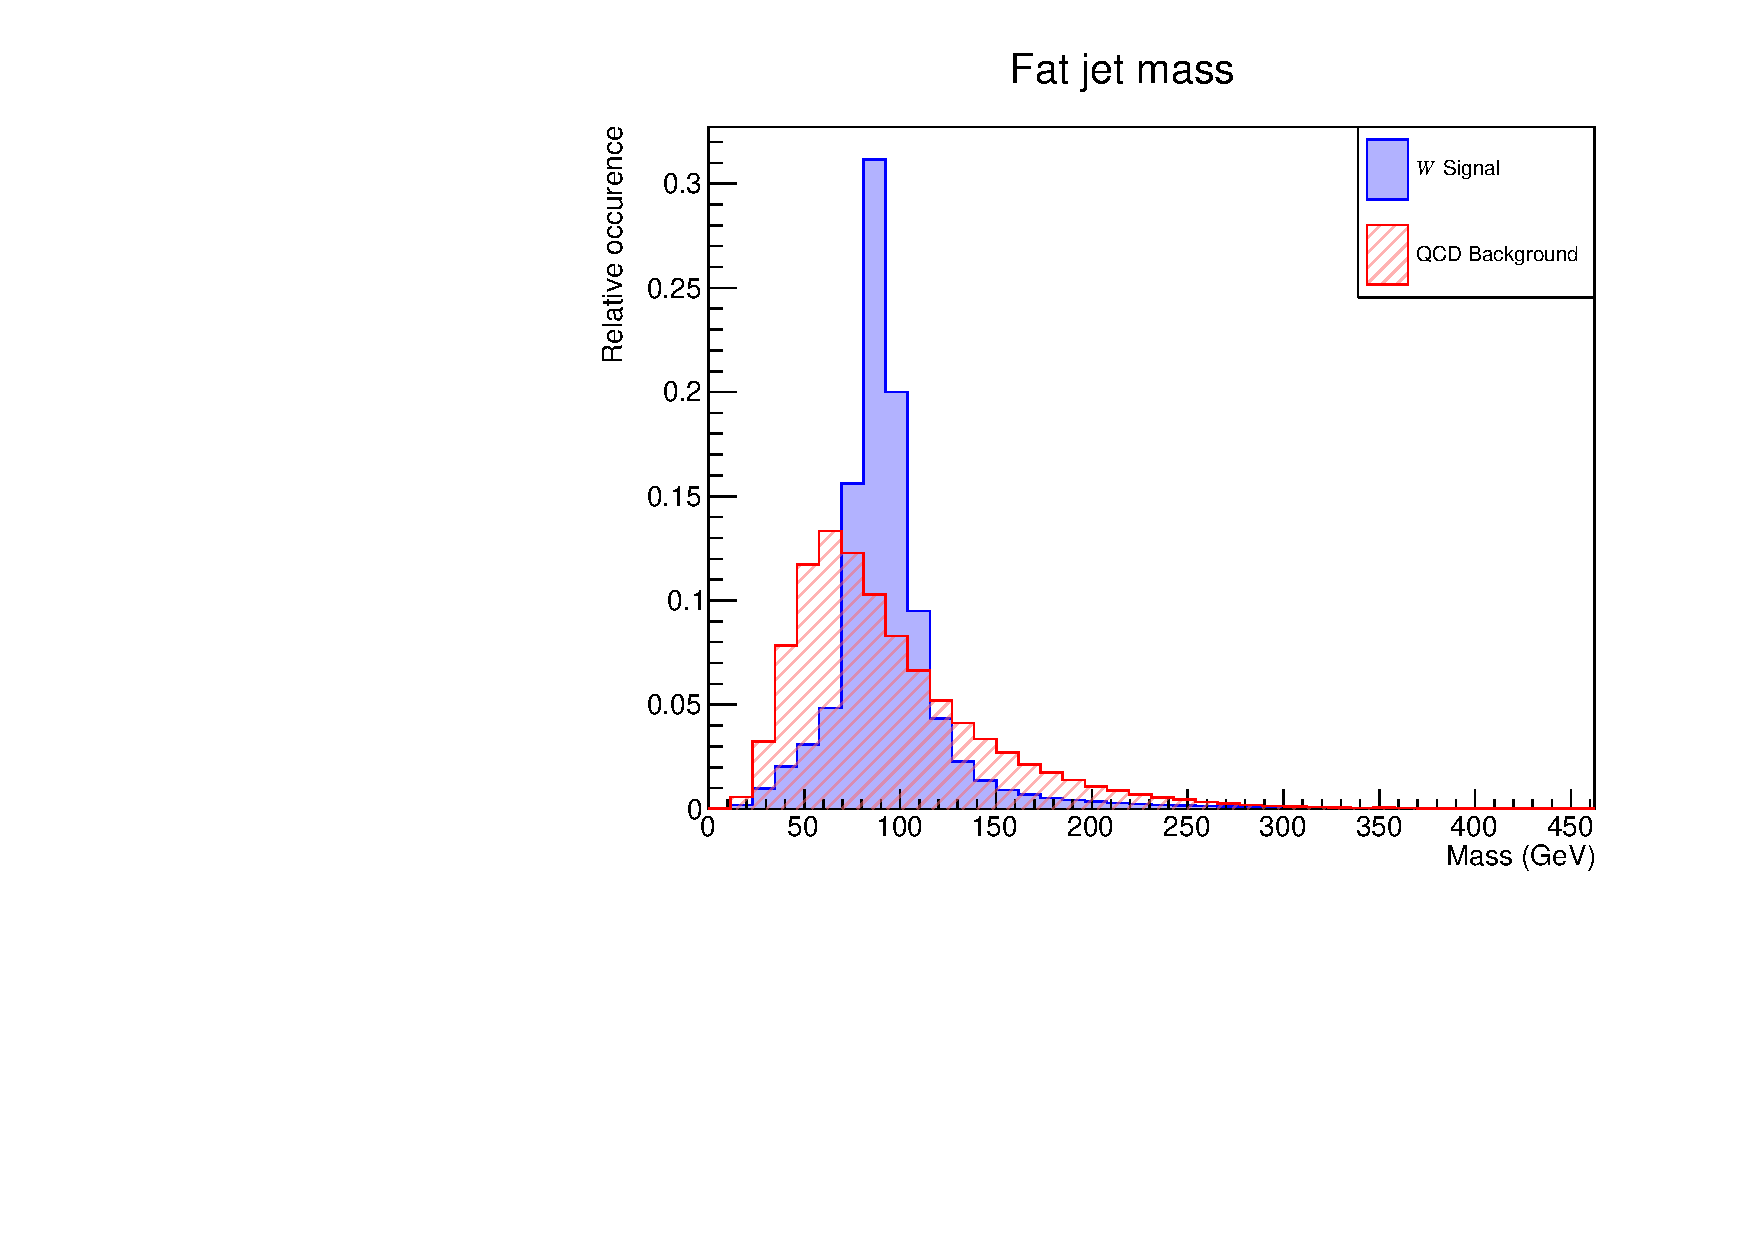
\includegraphics[width=0.8\textwidth]{../Figures/Results/W_distributions/W_mass_distribution.pdf}
          \caption{}
         \label{fig:W_distribution_mass}
     \end{subfigure}
     \caption{Distribution of (a)\;-\;(d) $\tau_N$, (e)\;-\;(g) $\tau_{N+1}/\tau_N$ ratios and (h) mass for the $W$ and QCD fat jets in the training sample events.}
        \label{fig:W_distributions}
\end{figure}

top signal distributions, in which $\tau_3/\tau_2$ presents a better discrimination. This is because fat jets originating from $W$ bosons are made up of two subjets while those originating from top quarks are made up of three. One common feature shared by the top and $W$ signals is that for higher $N$ values, the separation between signal and background for $\tau_{N+1}/\tau_N$ distributions vanishes. Because of this, the contribution of $\tau_N$ variables with high $N$ values to a classification would be negligible. Therefore, the set of $\tau_N$ variables used as input in the subsequent multivariate analysis consists of $\{\tau_1,\tau_2,\tau_3,\tau_4\}$.\\

For both the top and the $W$ signals, there is a clear distinction between the signal and background fat jet mass distributions, which are shown in figures \ref{fig:top_distributions}(h) and \ref{fig:W_distributions}(h). The signal distribution consists of a narrow peak around the top quark mass (the $W$ mass in the case of the $W$ signal) while the background one covers a wider range of mass values. This accounts for the good discriminant capabilities of this variable. For this reason, the jet mass is continuously used in jet tagging algorithms, and it is employed alongside the $N$-subjettiness variables in the multivariate analysis presented here. \\

From this point forward, the results of the machine learning implementation will be addressed. The performance of the different multivariate classifiers trained using \textsc{TMVA} will be analysed by looking at their respective Receiver Operating Characteristic (ROC) curve. The ROC curves are created by plotting the background rejection (the fraction of background events that are correctly identified as such by the classifier) versus the signal efficiency (the fraction of true signal events that are correctly identified by the classifier) as the discrimination threshold is varied. \\

The ROC curves for the different MV classifiers are presented in figure \ref{fig:ROC_classifiers}. As has been already mentioned, the variables used as input for the classifier training are the fat jet $\tau_N$ (with $N = 1,\dots,4$) and the fat jet mass. \\

\begin{figure}[H]
     \centering
     \begin{subfigure}[h]{0.49\textwidth}
         \centering
         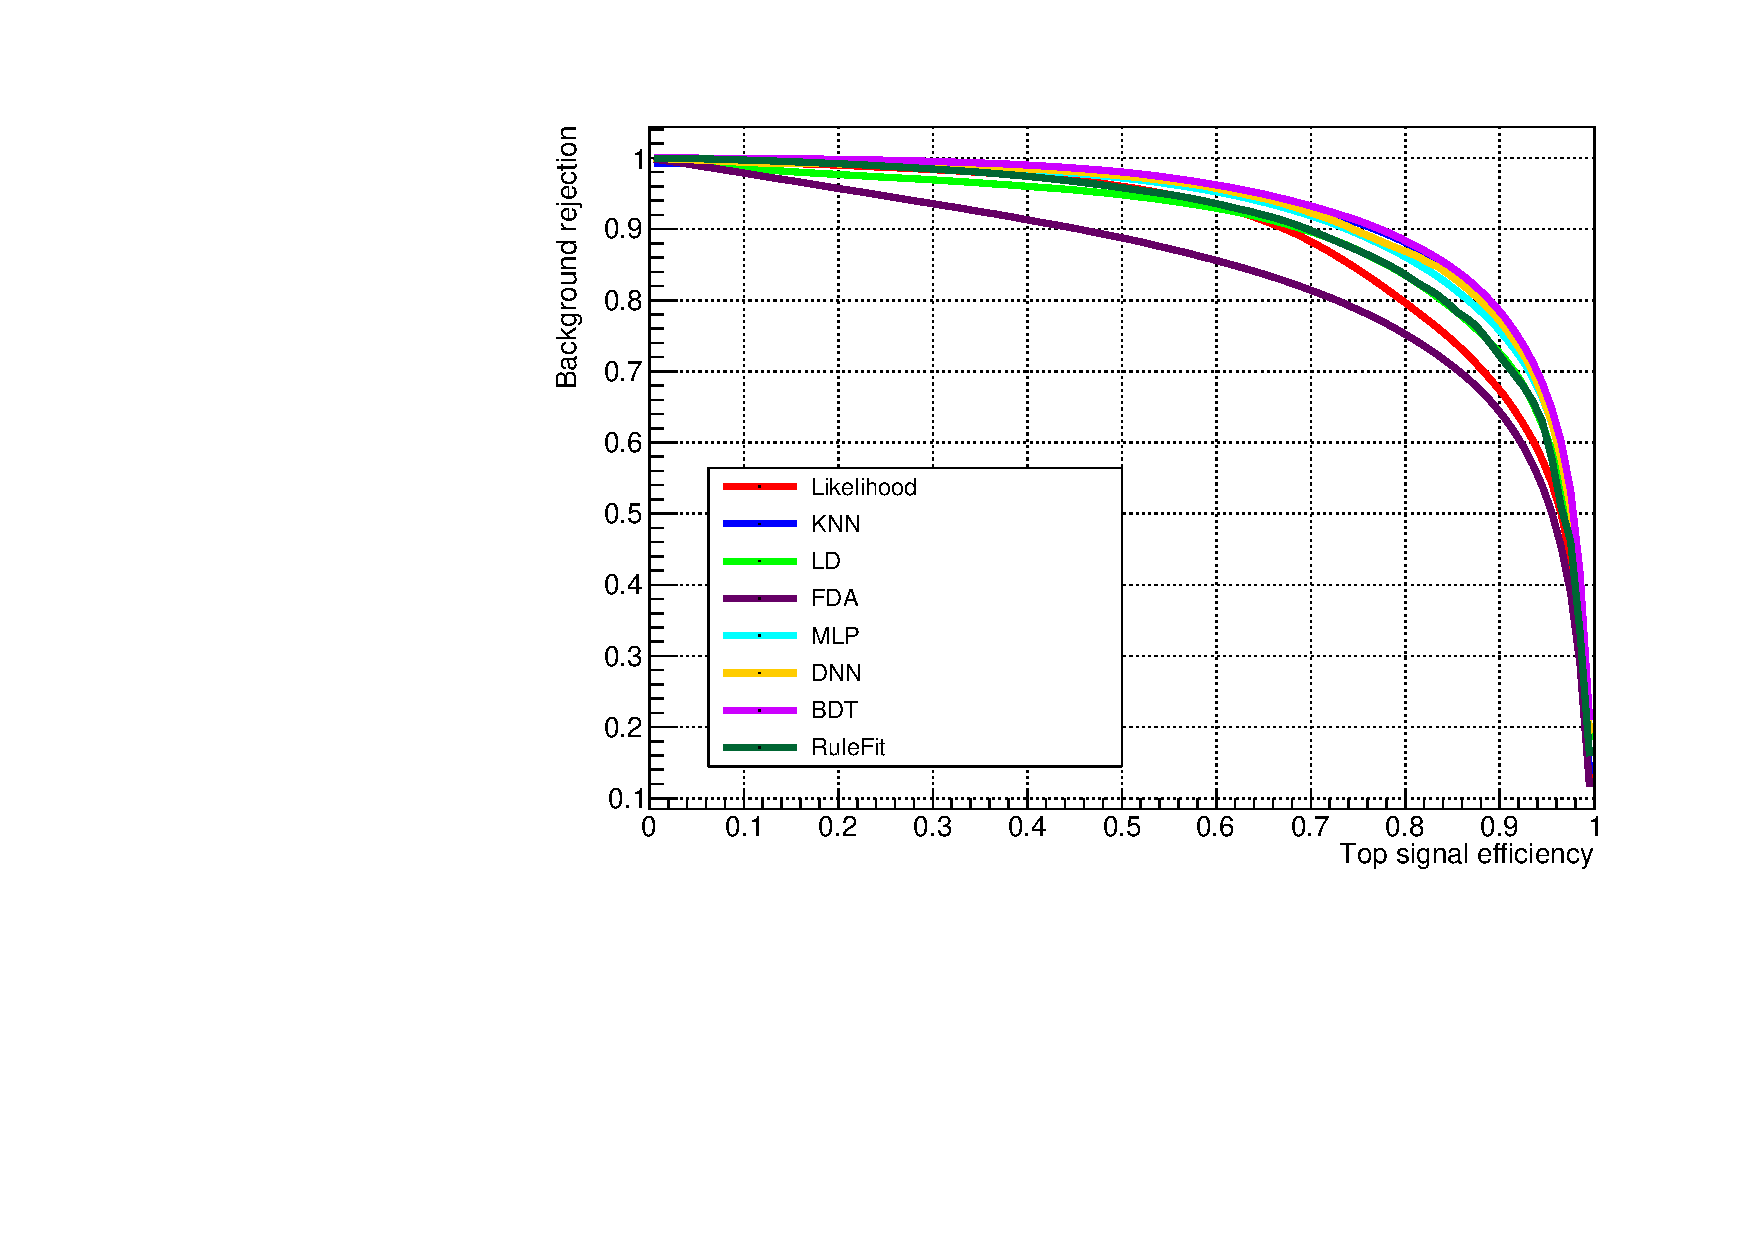
\includegraphics[width=\textwidth]{../Figures/Results/multiple_classifiers/top_multipleclassifiers.pdf}
          \caption{}
         \label{fig:top_multipleclassifiers}
     \end{subfigure}
     \begin{subfigure}[h]{0.49\textwidth}
         \centering
         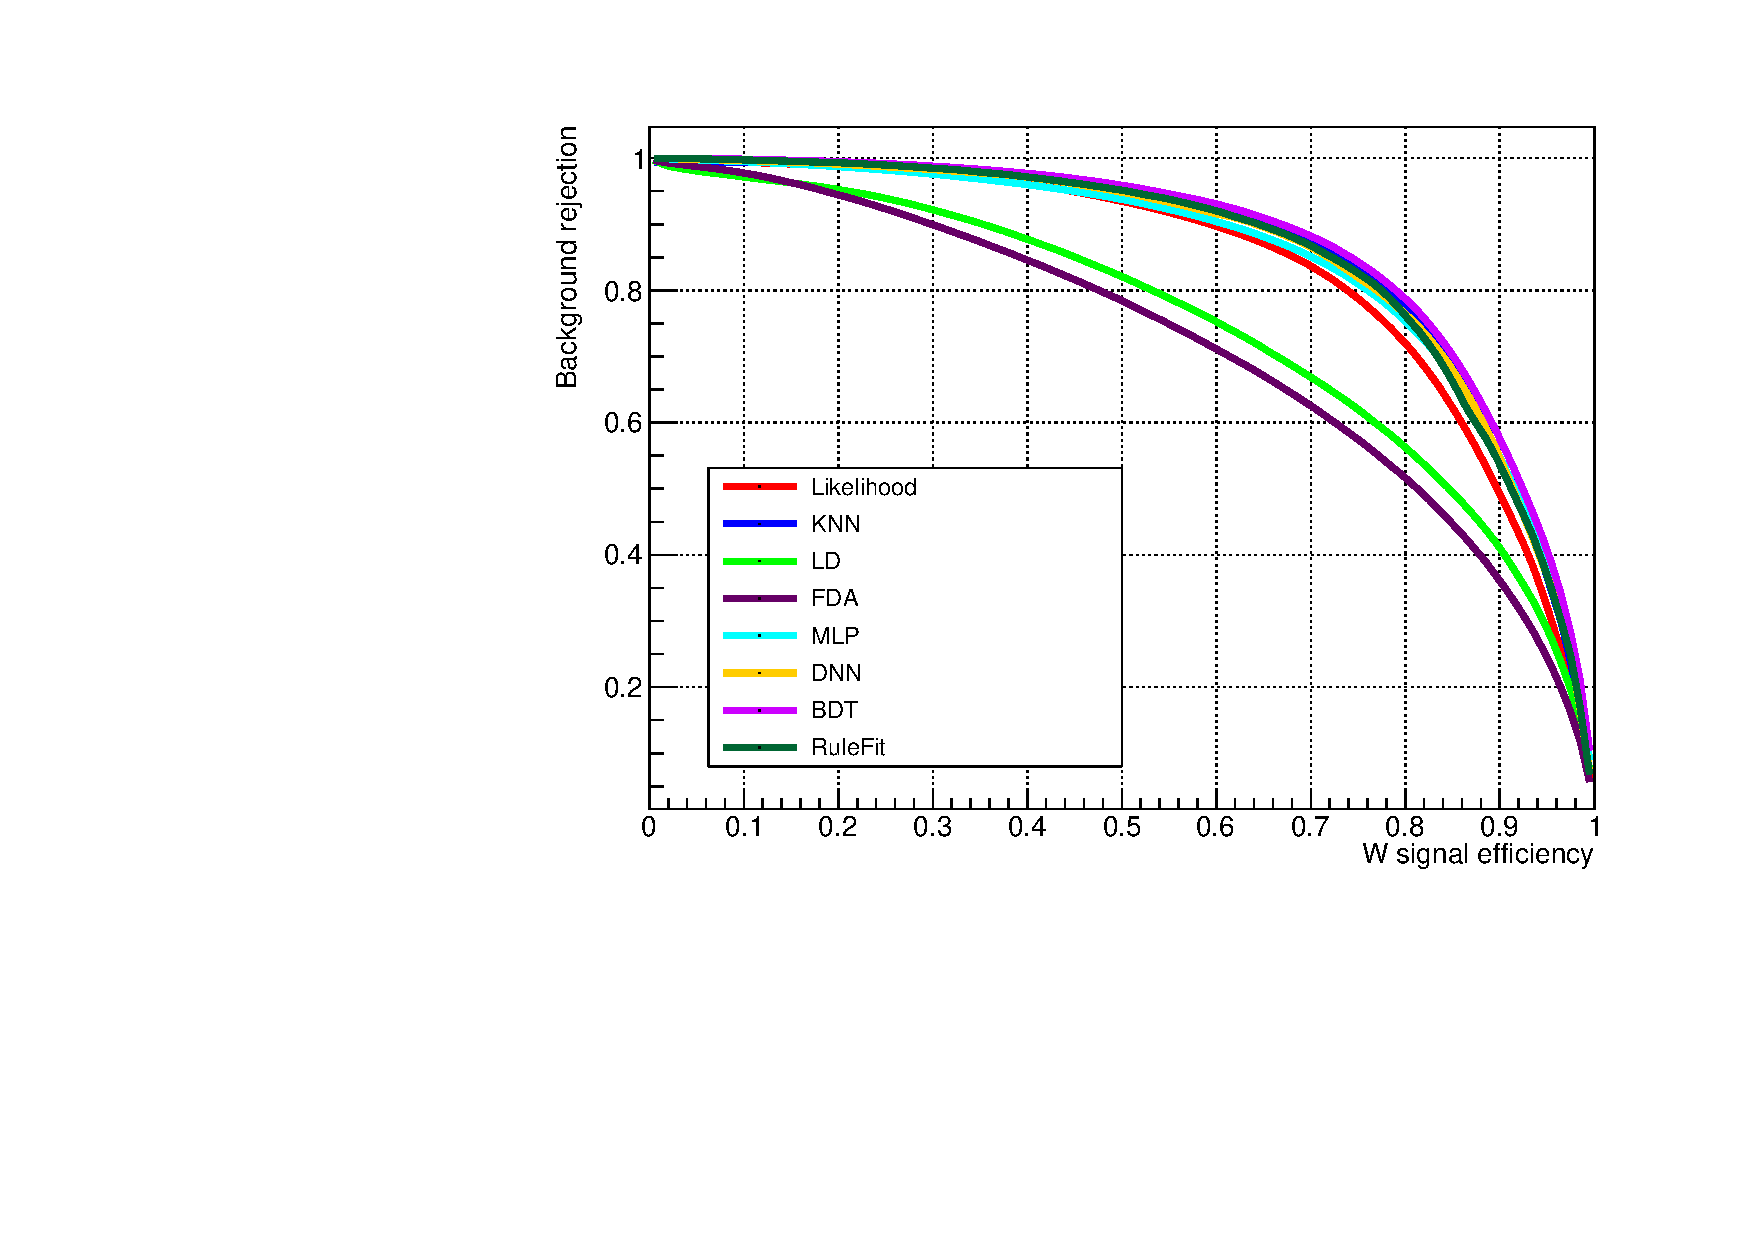
\includegraphics[width=\textwidth]{../Figures/Results/multiple_classifiers/W_multipleclassifiers.pdf}
          \caption{}
         \label{fig:W_multipleclassifiers}
     \end{subfigure}
     \caption{ROC curves of the different multivariate classifiers trained for (a) boosted top tagging (b) boosted $W$ tagging.}
     \label{fig:ROC_classifiers}
\end{figure}

The area under the ROC curve (AUC) is a commonly used metric for evaluating the performance of a classifier algorithm. A higher AUC value indicates a better classifier performance, with a value of 1.0 denoting a perfect classification (total background rejection for a maximum signal efficiency). The AUC values obtained for both boosted top tagging and boosted $W$ tagging are presented in table \ref{tab:AUC_values}. \\


\begin{table}[h]
\centering
\begin{tabular}{|c|c|c|}
\hline
MVA Method & AUC (Top signal) & AUC ($W$ Signal) \\ \hline
BDT        & 0.925            & 0.871          \\ \hline
KNN        & 0.920            & 0.862          \\ \hline
DNN        & 0.917            & 0.858          \\ \hline
MLP        & 0.915            & 0.851          \\ \hline
RuleFit    & 0.899            & 0.858          \\ \hline
LD         & 0.892            & 0.751          \\ \hline
Likelihood & 0.887            & 0.838          \\ \hline
FDA        & 0.840            & 0.723          \\ \hline
\end{tabular}
\caption{Area under the ROC curve of the different multivariate classifiers used.}
\label{tab:AUC_values}
\end{table}

As evidenced by the AUC values obtained, the classifiers perform better overall in the tagging of top quarks than in that of $W$ bosons. This was expected, since the substructure of fat jets originating from top quarks is somewhat more distinguishable. It is worth pointing out that the best tagging performance was achieved by the boosted decision tree in both cases. Therefore, it is chosen as the preferred classifier in subsequent analyses. Despite the fact that its performance is slightly worse, the DNN also continues to be considered as a deep learning alternative alongside the BDT method.\\ 

Before moving forward it is important to verify that the chosen classifiers are not being overtrained. In order to do so, the classifier response distributions for signal and background are plotted for both training and test data in figure \ref{fig:overtraining}. As can be seen from the figure, the training and test distributions are very similar in all cases, indicating that overtraining has been avoided. \\

\begin{figure}[H]
     \centering
     \begin{subfigure}[h]{0.49\textwidth}
         \centering
         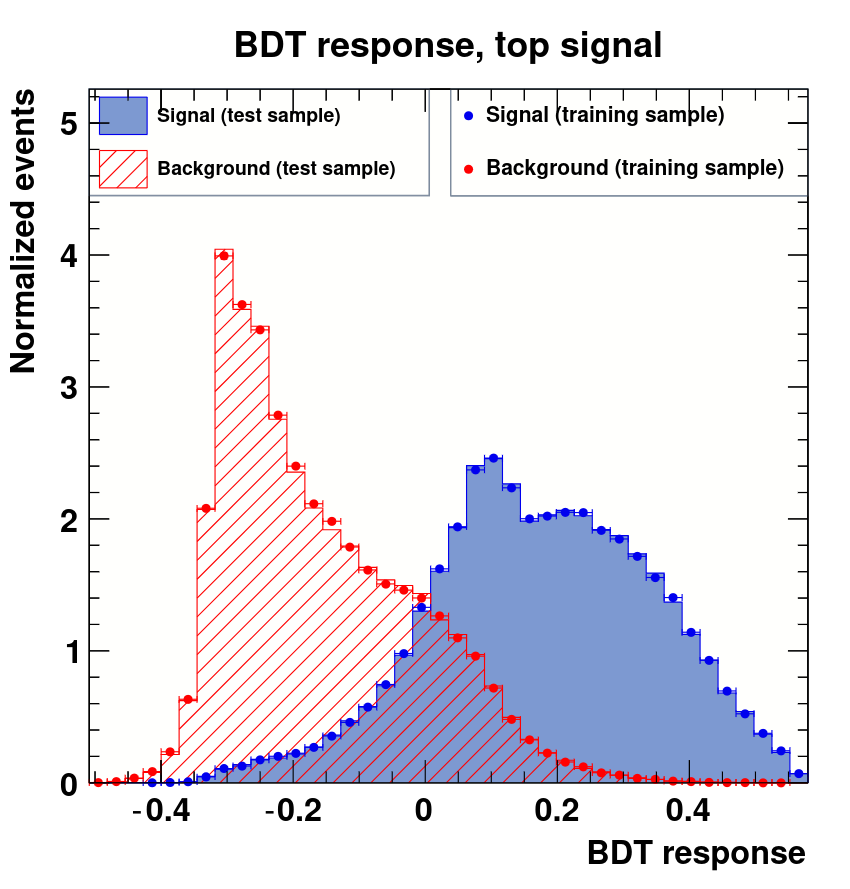
\includegraphics[width=0.8\textwidth]{../Figures/Results/overtraining/top_overtraining_BDT.png}
          \caption{}
         \label{fig:top_BDT_overtraining}
     \end{subfigure}
     \begin{subfigure}[h]{0.49\textwidth}
         \centering
         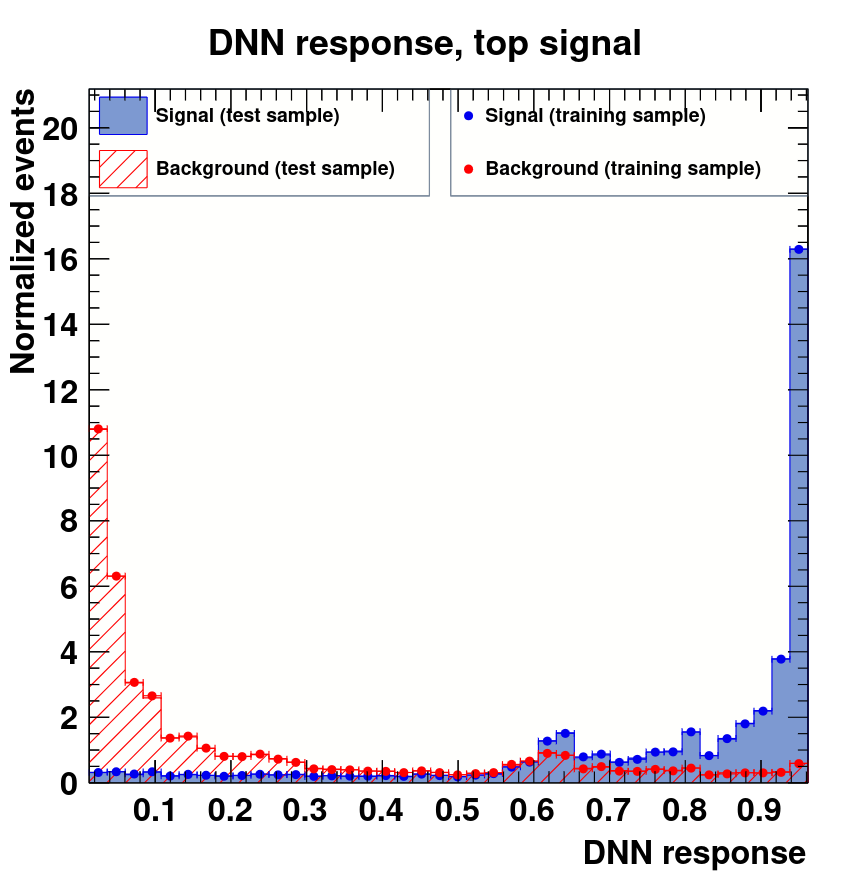
\includegraphics[width=0.8\textwidth]{../Figures/Results/overtraining/top_overtraining_DNN.png}
          \caption{}
         \label{fig:top_DNN_overtraining}
     \end{subfigure}
     \par\bigskip
     \begin{subfigure}[h]{0.49\textwidth}
         \centering
         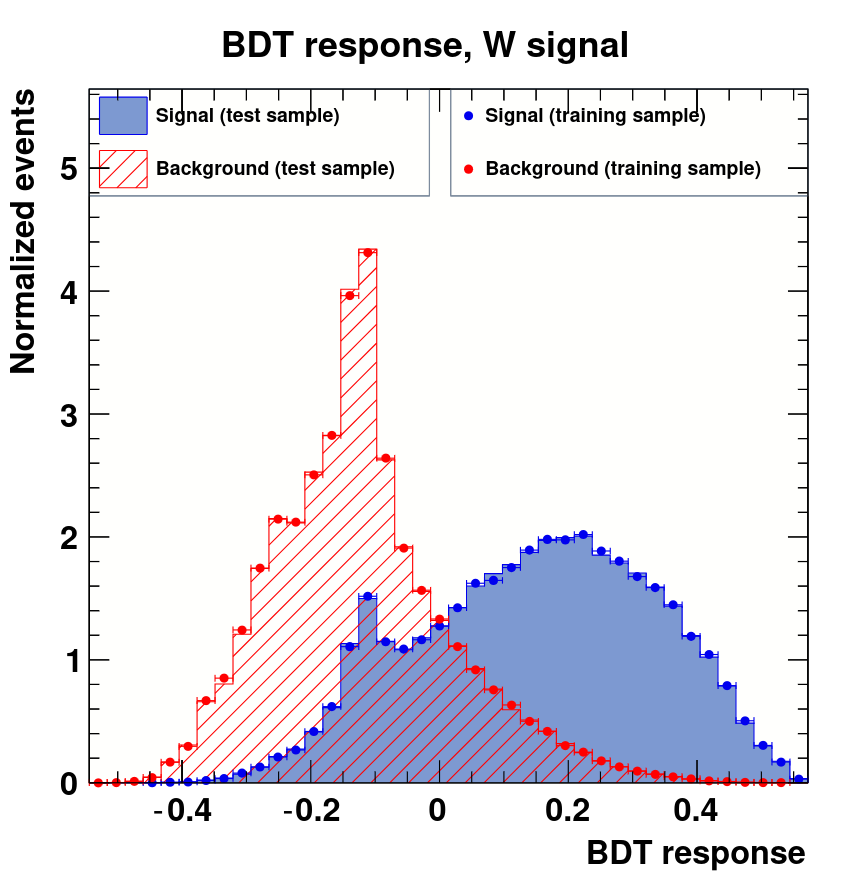
\includegraphics[width=0.8\textwidth]{../Figures/Results/overtraining/W_overtraining_BDT.png}
          \caption{}
         \label{fig:W_BDT_overtraining}
     \end{subfigure}
     \begin{subfigure}[h]{0.49\textwidth}
         \centering
         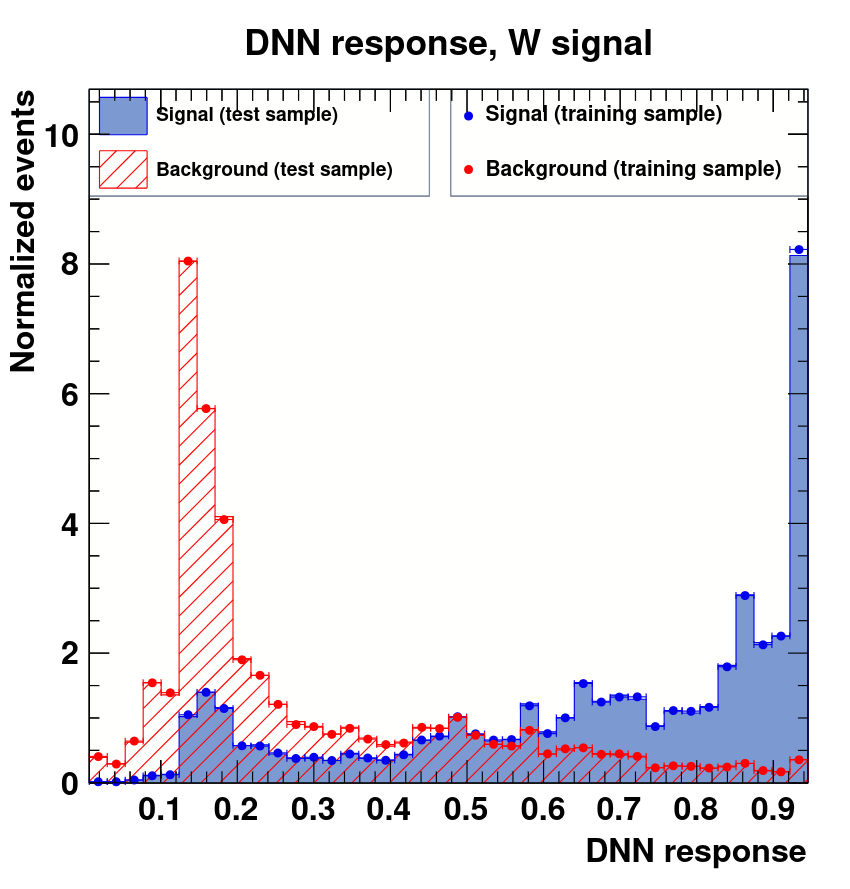
\includegraphics[width=0.8\textwidth]{../Figures/Results/overtraining/W_overtraining_DNN.png}
          \caption{}
         \label{fig:W_DNN_overtraining}
     \end{subfigure}
     \caption{Distribution of the BDT and DNN classifier responses for training and test data in (a) - (b) boosted top tagging (c) - (d) boosted $W$ tagging.}
        \label{fig:overtraining}
\end{figure}

Up until now the fat jet mass has been used alongside the $N$-subjettiness variables as an input variable in the classifier training. This is because the mass works as a great discriminant variable, as has been shown already. However, in order to further examine the tagging performance of the $N$-subjettiness jet shape, a classification based on the $\tau_N$ variables alone is carried out. The ROC curves obtained both with and without using fat jet mass information for the classification are plotted for each case in figure \ref{fig:ROC_mass_nomass}. \\

\begin{figure}[h]
     \centering
     \begin{subfigure}[h]{0.49\textwidth}
         \centering
         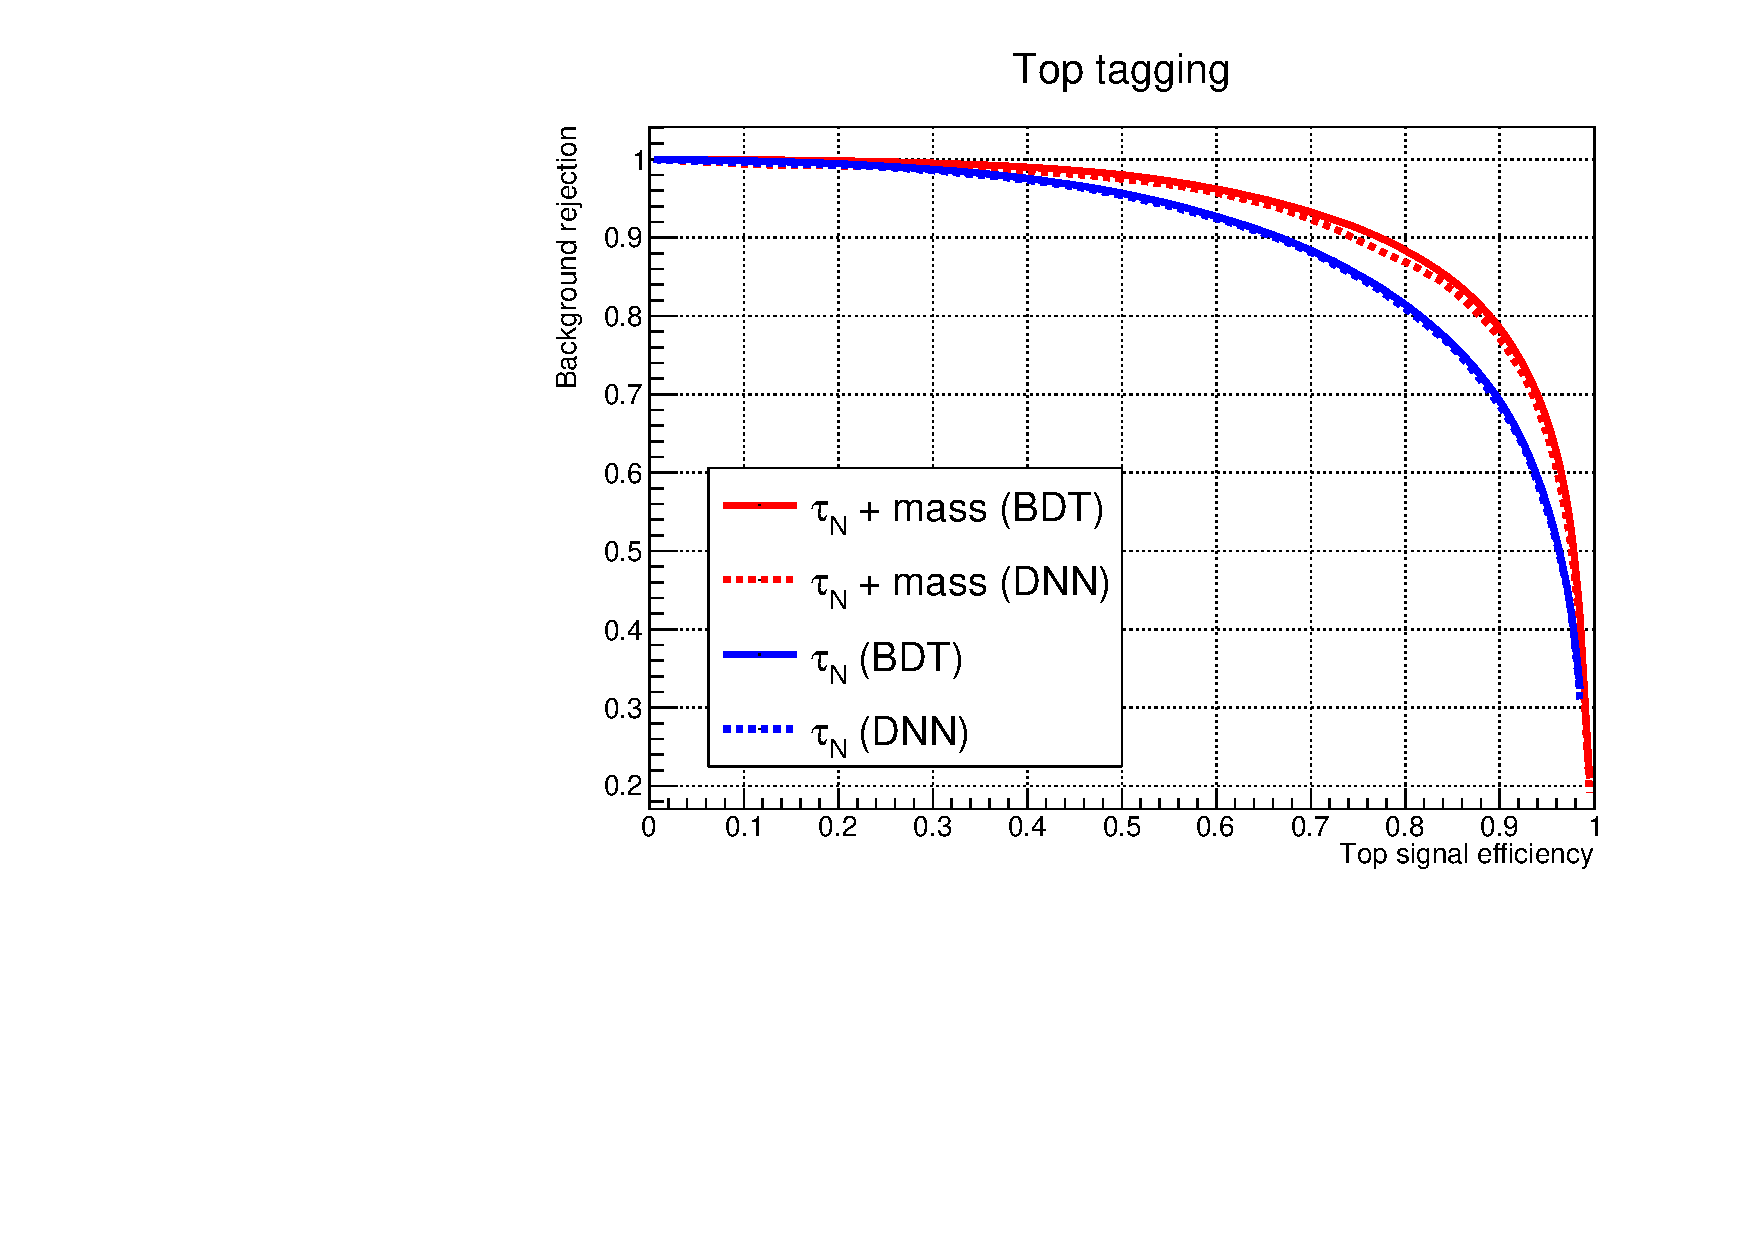
\includegraphics[width=\textwidth]{../Figures/Results/mass/top_mass_nomass.pdf}
          \caption{}
         \label{fig:top_mass_nomass}
     \end{subfigure}
     \begin{subfigure}[h]{0.49\textwidth}
         \centering
         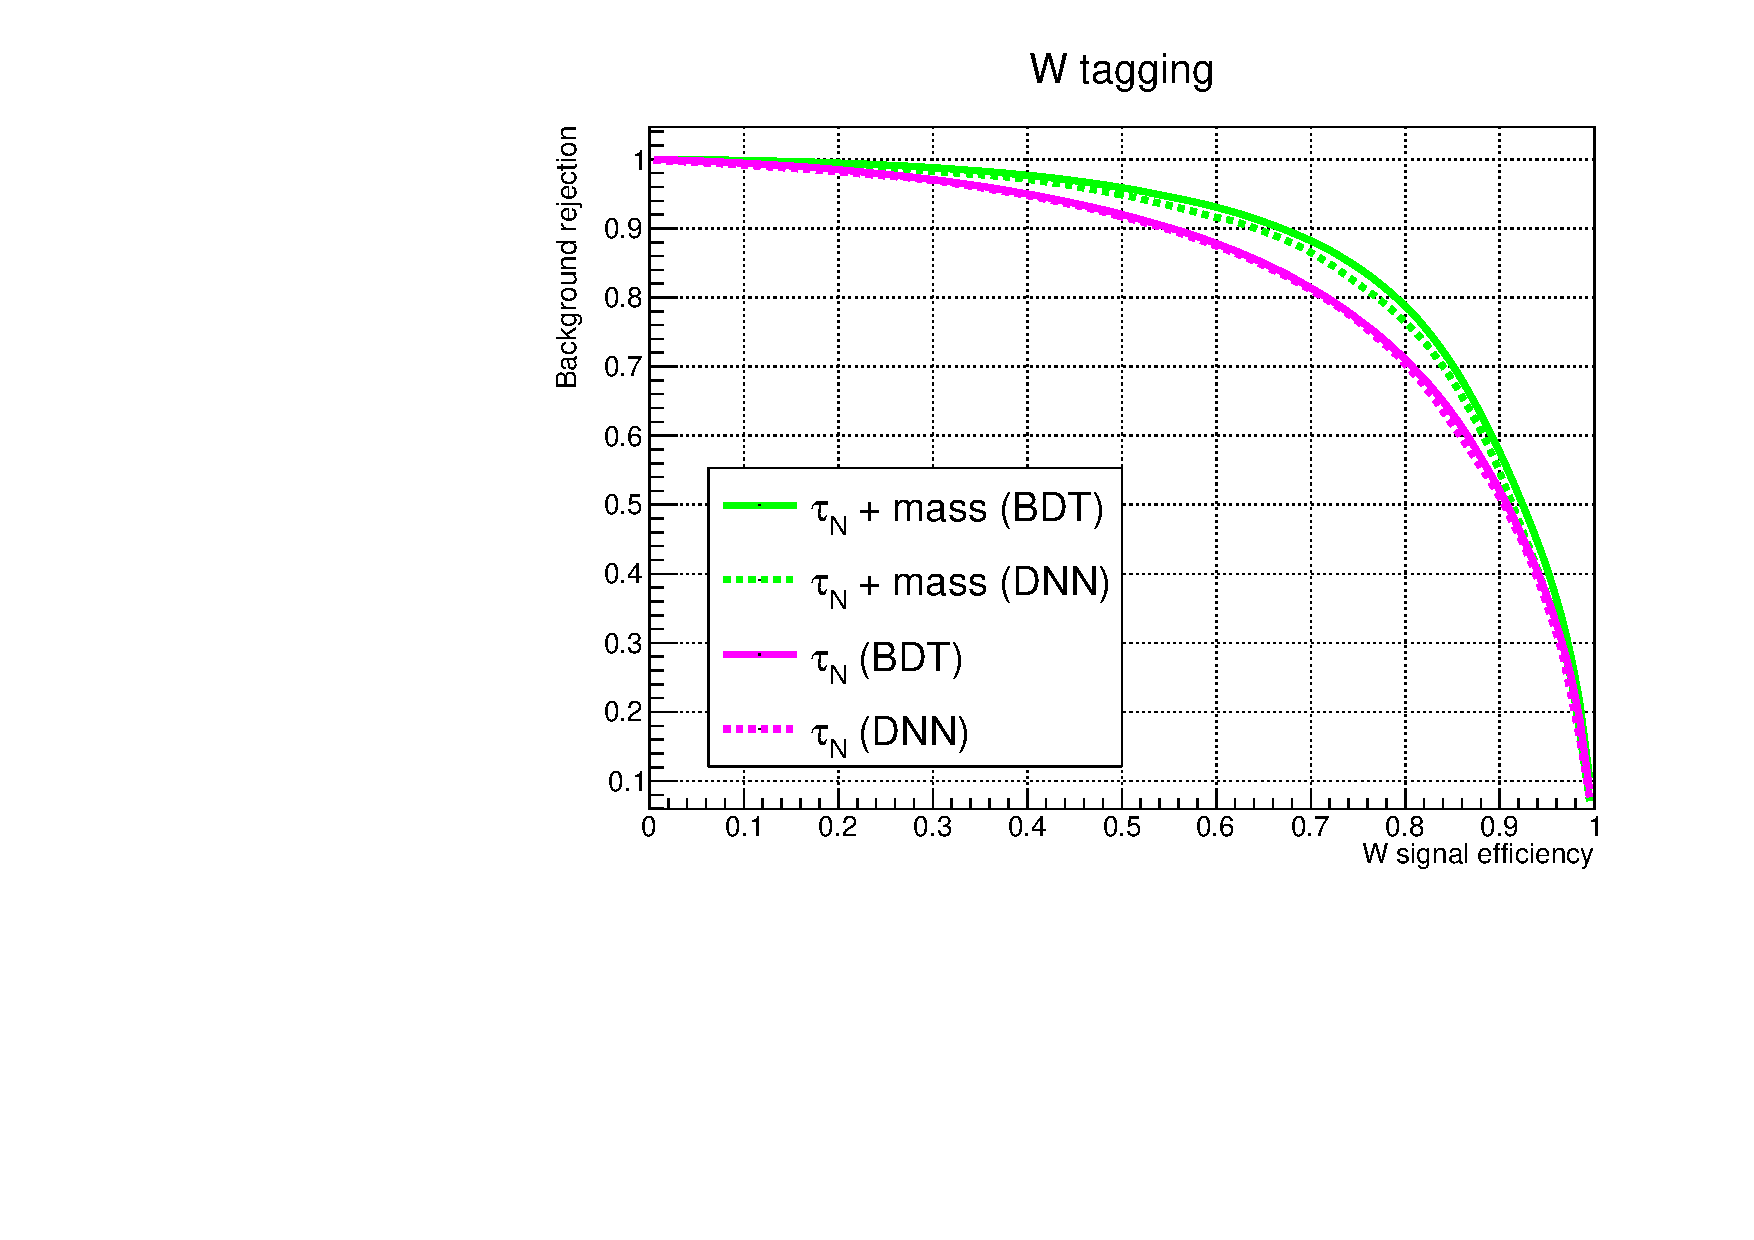
\includegraphics[width=\textwidth]{../Figures/Results/mass/W_mass_nomass.pdf}
          \caption{}
         \label{fig:W_mass_nomass}
     \end{subfigure}
     \caption{ROC curves for (a) boosted top tagging (b) boosted $W$ tagging with and without including the fat jet mass as an input variable.}
     \label{fig:ROC_mass_nomass}
\end{figure}

As evidenced by the respective ROC curves, the fat jet mass has a noticeable contribution to the tagging performance. This corroborates that using both substructure variables in conjunction is optimal. However, it is also worth noticing the remarkable discriminating job that the $\tau_N$ can do on their own, which confirms that they are not dependant on the mass in order to carry out a classification. \\

So far the full set of $\tau_N$ values with $N = 1,\dots,4$ have been used. The impact of the number of $\tau_N$ variables used as input for the classifier training will now be addressed. In order to do so, the model is trained first using only the fat jet $\tau_1$ value (plus the fat jet mass) then the following $\tau_N$ variables are added, one at a time until $\tau_4$ is reached and the original set is achieved. The ROC curves obtained through this process are presented in figure \ref{fig:ROC_multibody}. \\

\begin{figure}[h]
     \centering
     \begin{subfigure}[h]{0.49\textwidth}
         \centering
         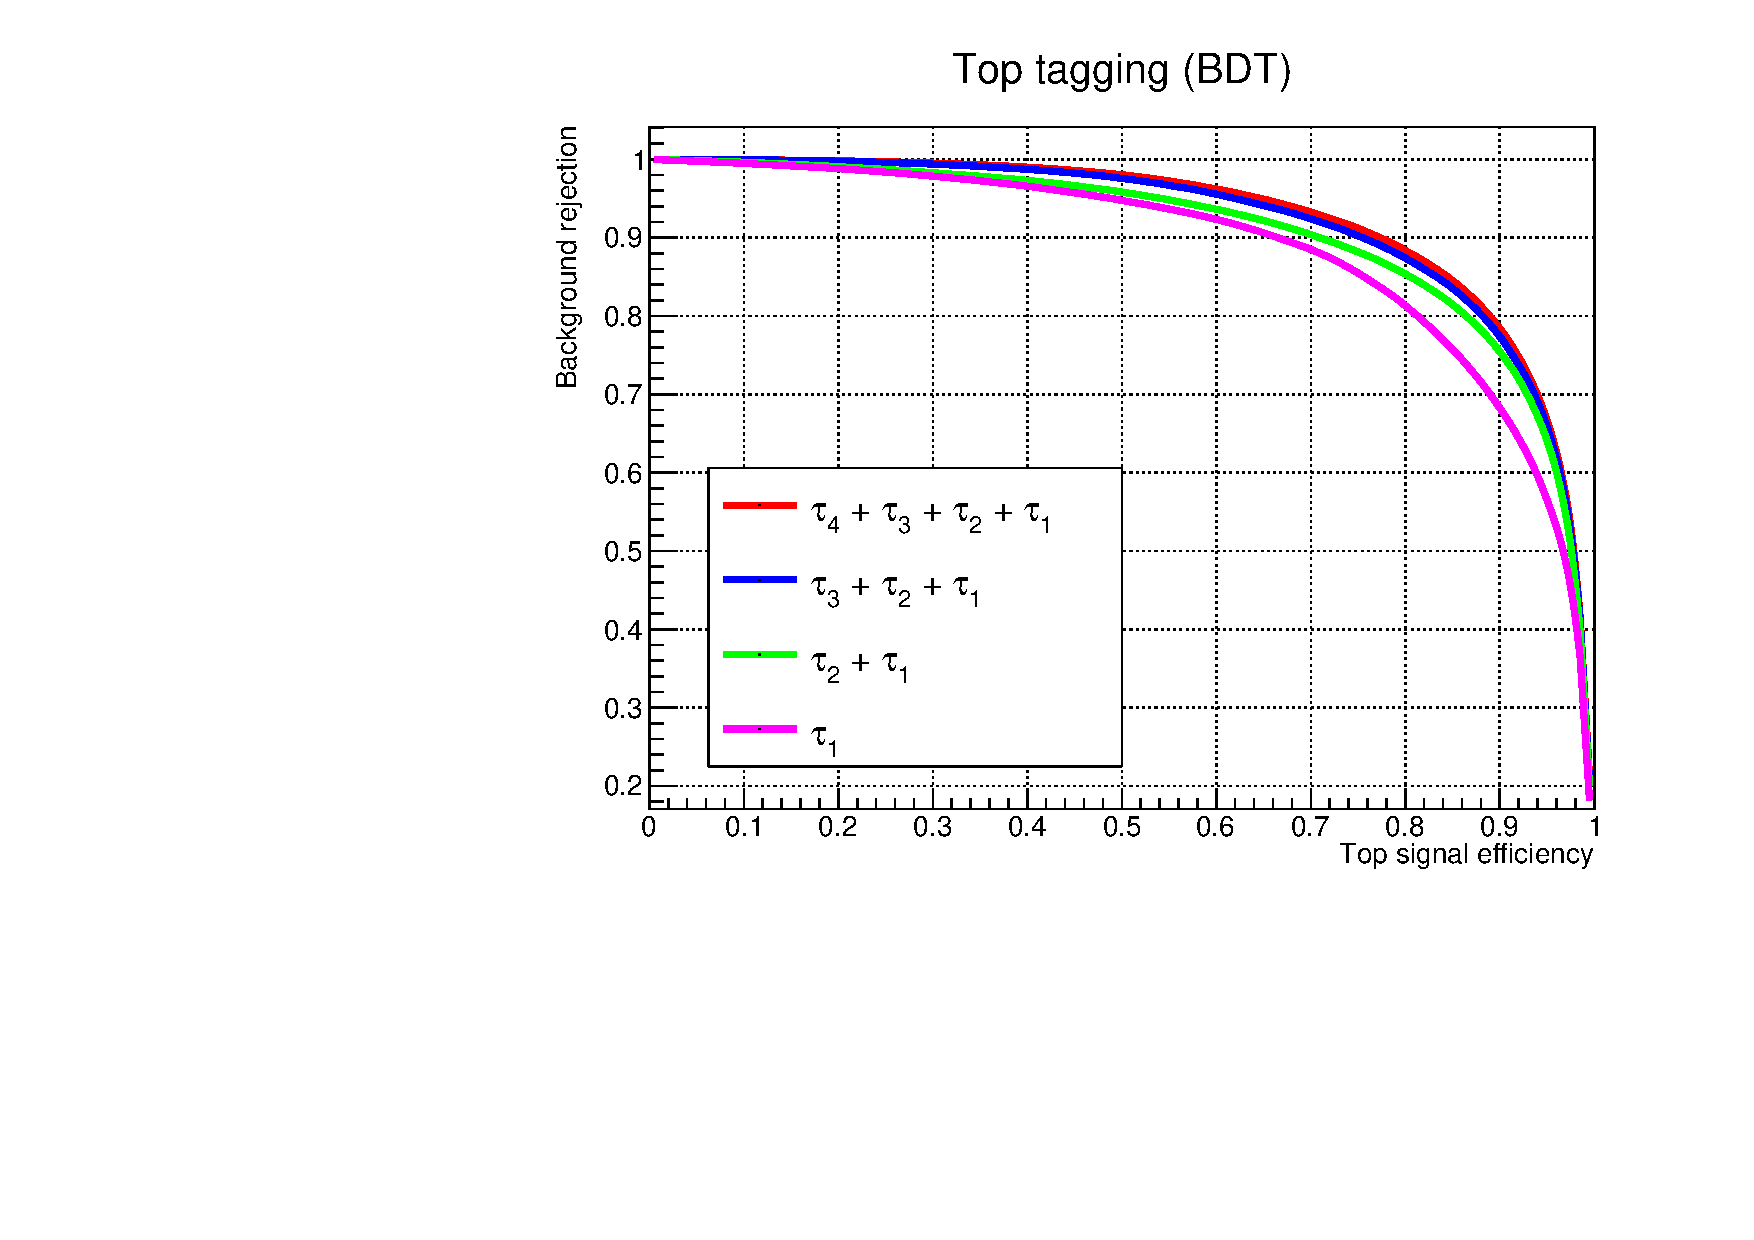
\includegraphics[width=\textwidth]{../Figures/Results/multibody/top_multibody.pdf}
          \caption{}
         \label{fig:top_multibody}
     \end{subfigure}
     \begin{subfigure}[h]{0.49\textwidth}
         \centering
         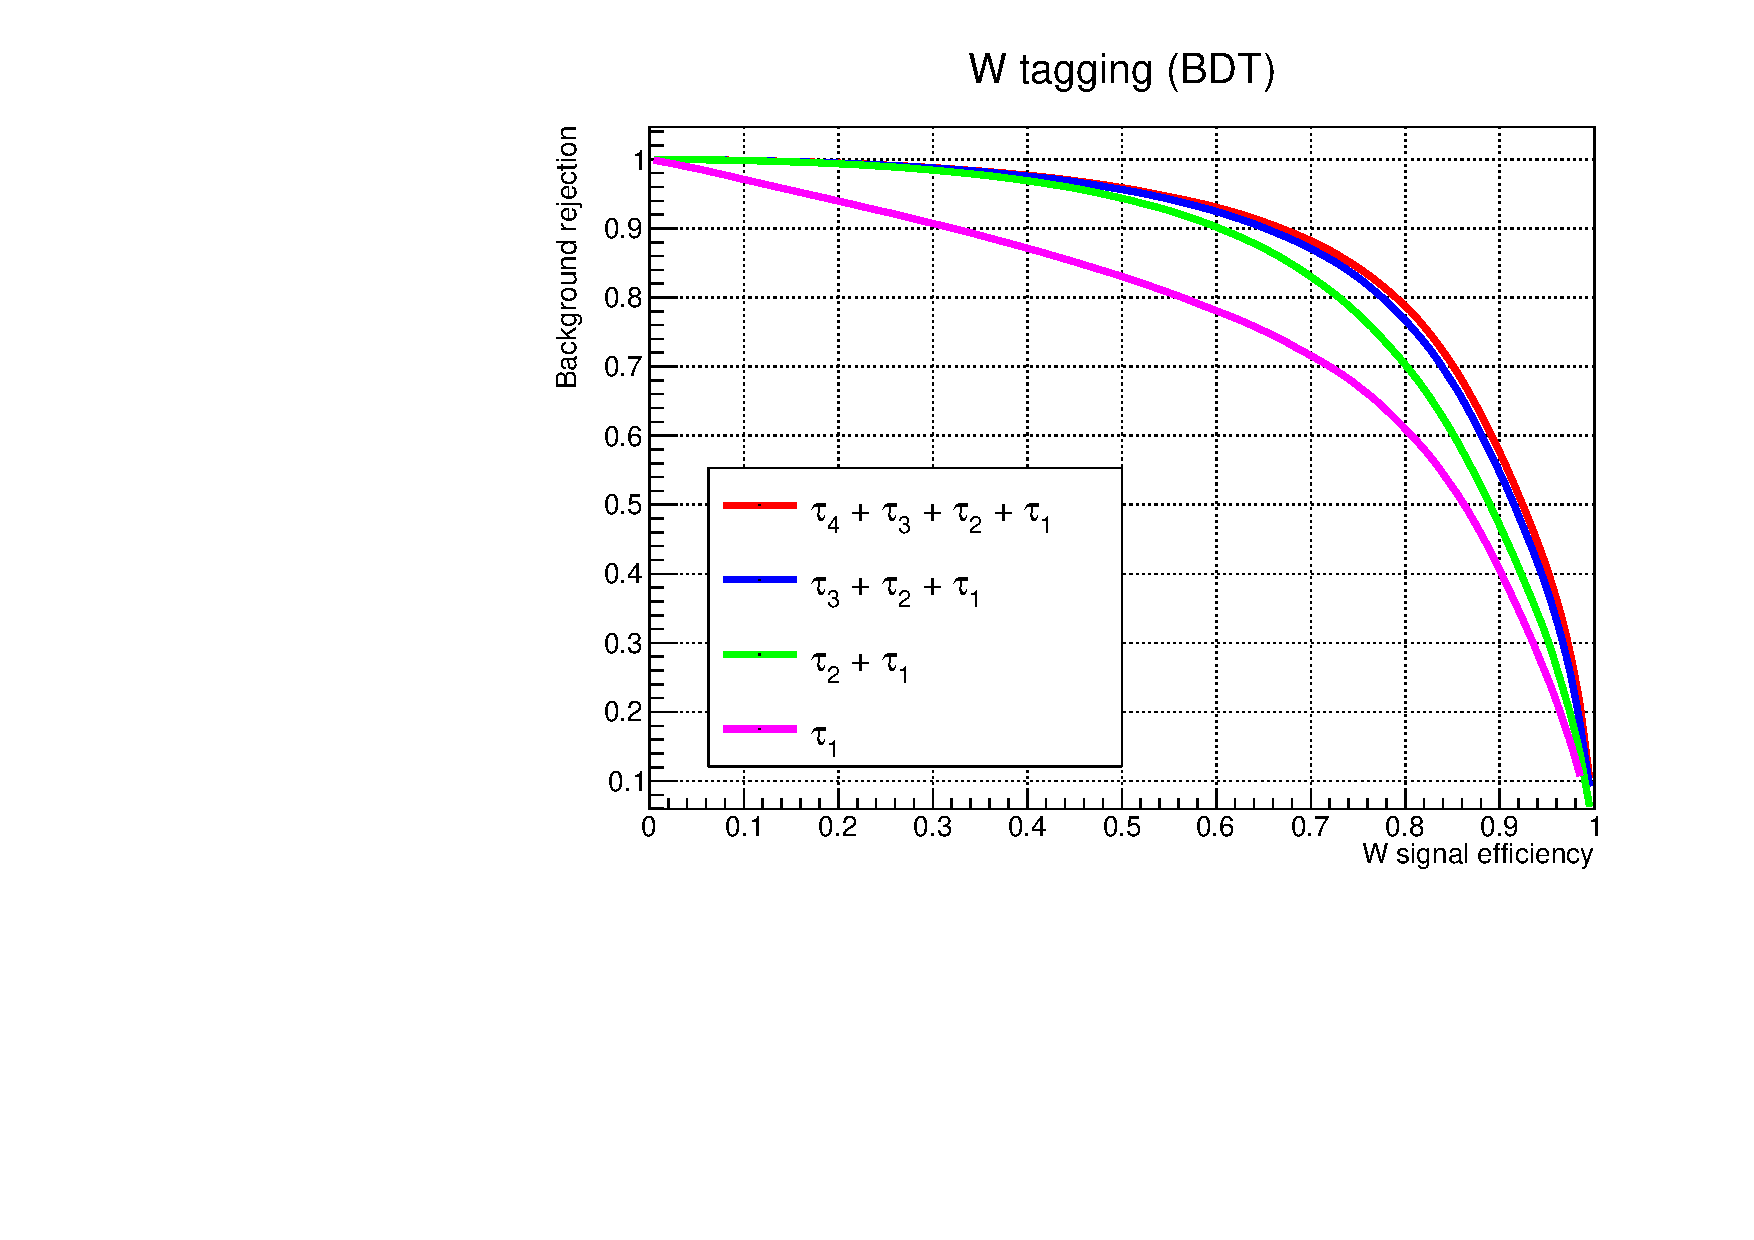
\includegraphics[width=\textwidth]{../Figures/Results/multibody/W_multibody.pdf}
          \caption{}
         \label{fig:W_multibody}
     \end{subfigure}
     \caption{ROC curves for (a) boosted top tagging (b) boosted $W$ tagging using different number of fat jet $\tau_N$ variables (and fat jet mass) as input.}
     \label{fig:ROC_multibody}
\end{figure}

This time the tagging performance was plotted using the BDT method only for simplicity. However, the same behaviour is observed when the trained algorithm is the DNN. As the number of $\tau_N$ inputs is increased, the gain in performance decreases notably to the point where the model gets saturated with information. This supports the initial decision of selecting the full set of $\tau_N$ input variables as those up to $N = 4$. \\

Finally, the tagging performance of the substructure variables used until now will be compared to that of other variables which are commonly used in multiple tagging methods. The variables considered for the comparison are those related to the constituents of the jets (in this case of the fat jets) being reconstructed. In this instance, the fat jet constituents refer to the calorimeter tower information, namely the total number of towers in each fat jet, the number of those towers with $E_T > 20$\;GeV and their cinematic information ($E_T$, $\eta$ and $\phi$ values). The exact same machine learning implementation used previously for the tagging based on substructure variables is used once again taking these constituent variables as an input. The tagging performance obtained in this way can be seen in figure \ref{fig:ROC_constituents}, together with the performance obtained earlier using substructure information.\\  

\begin{figure}[h]
     \centering
     \begin{subfigure}[h]{0.49\textwidth}
         \centering
         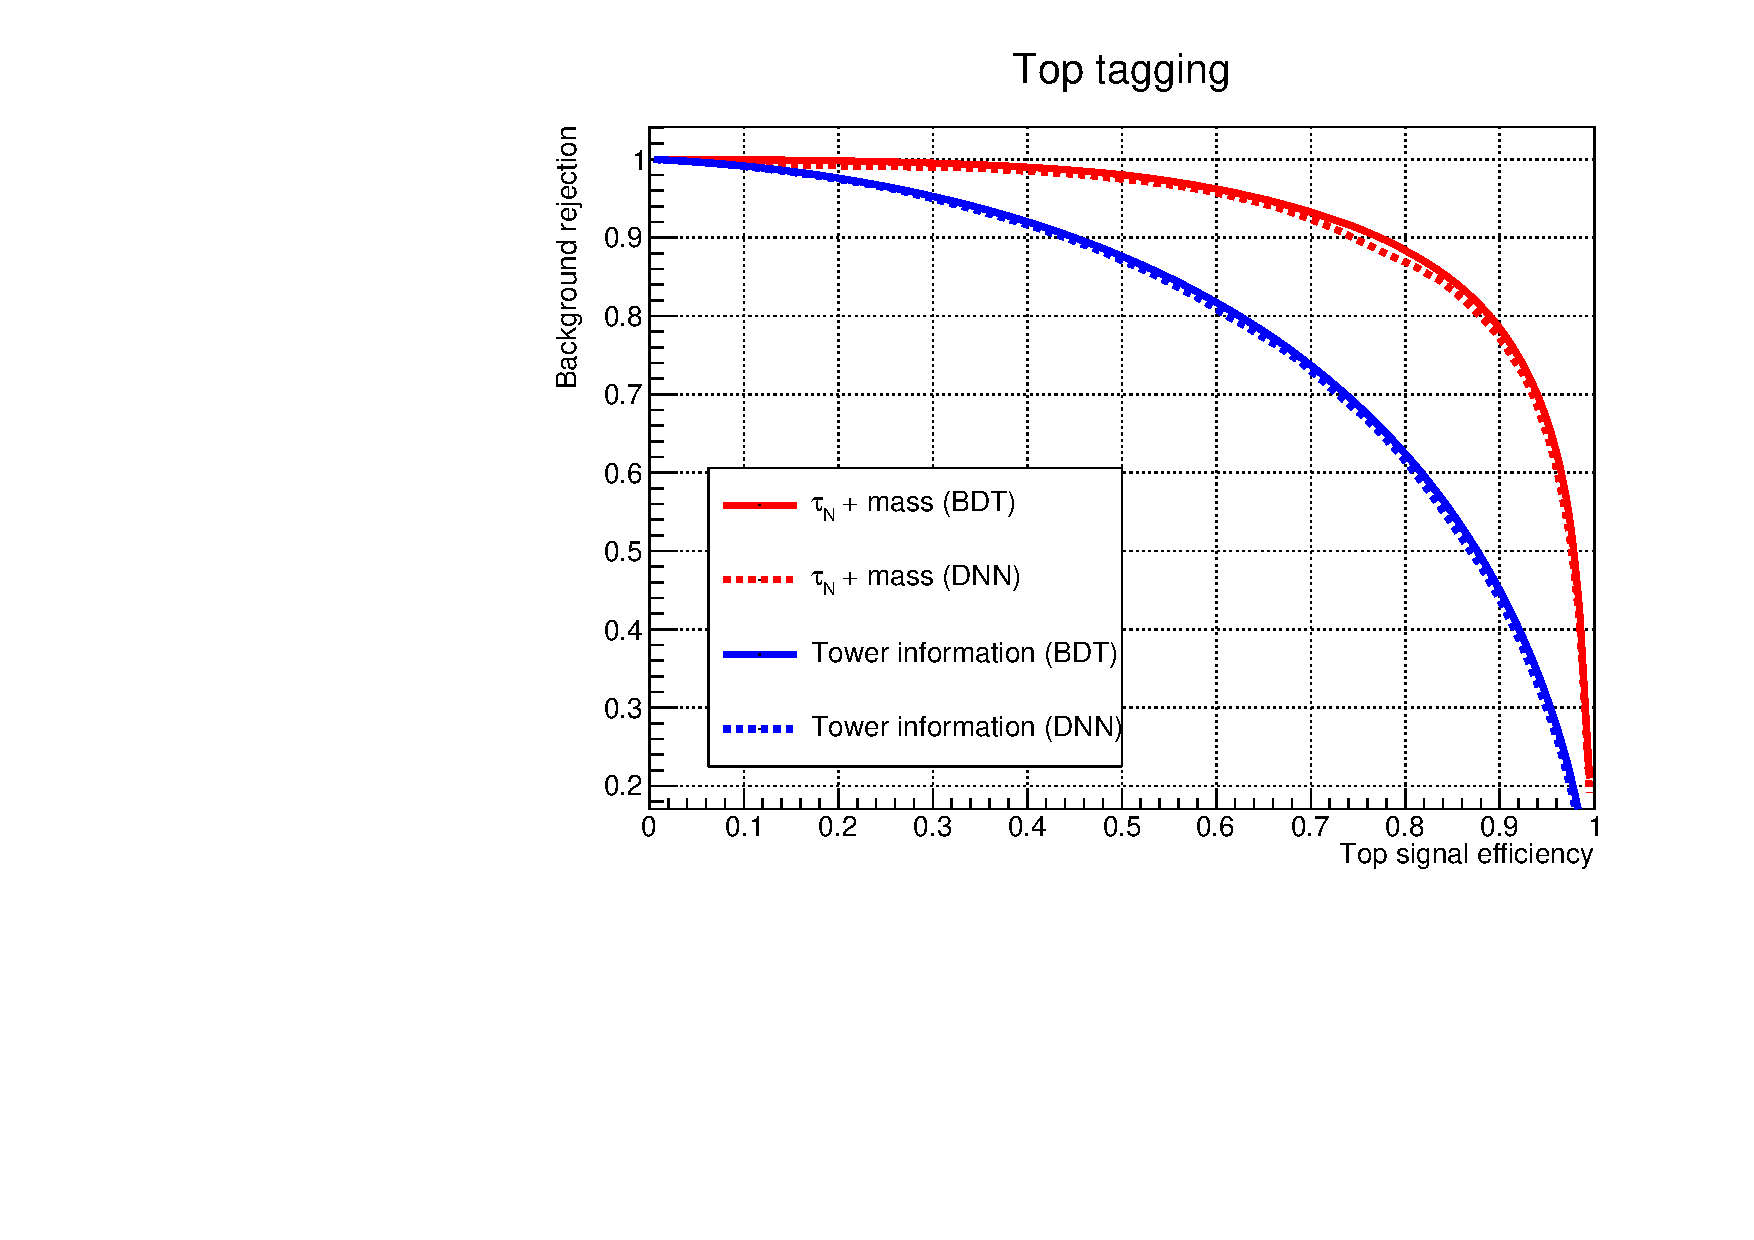
\includegraphics[width=\textwidth]{../Figures/Results/constituents/top_constituents.pdf}
          \caption{}
         \label{fig:top_constituents}
     \end{subfigure}
     \begin{subfigure}[h]{0.49\textwidth}
         \centering
         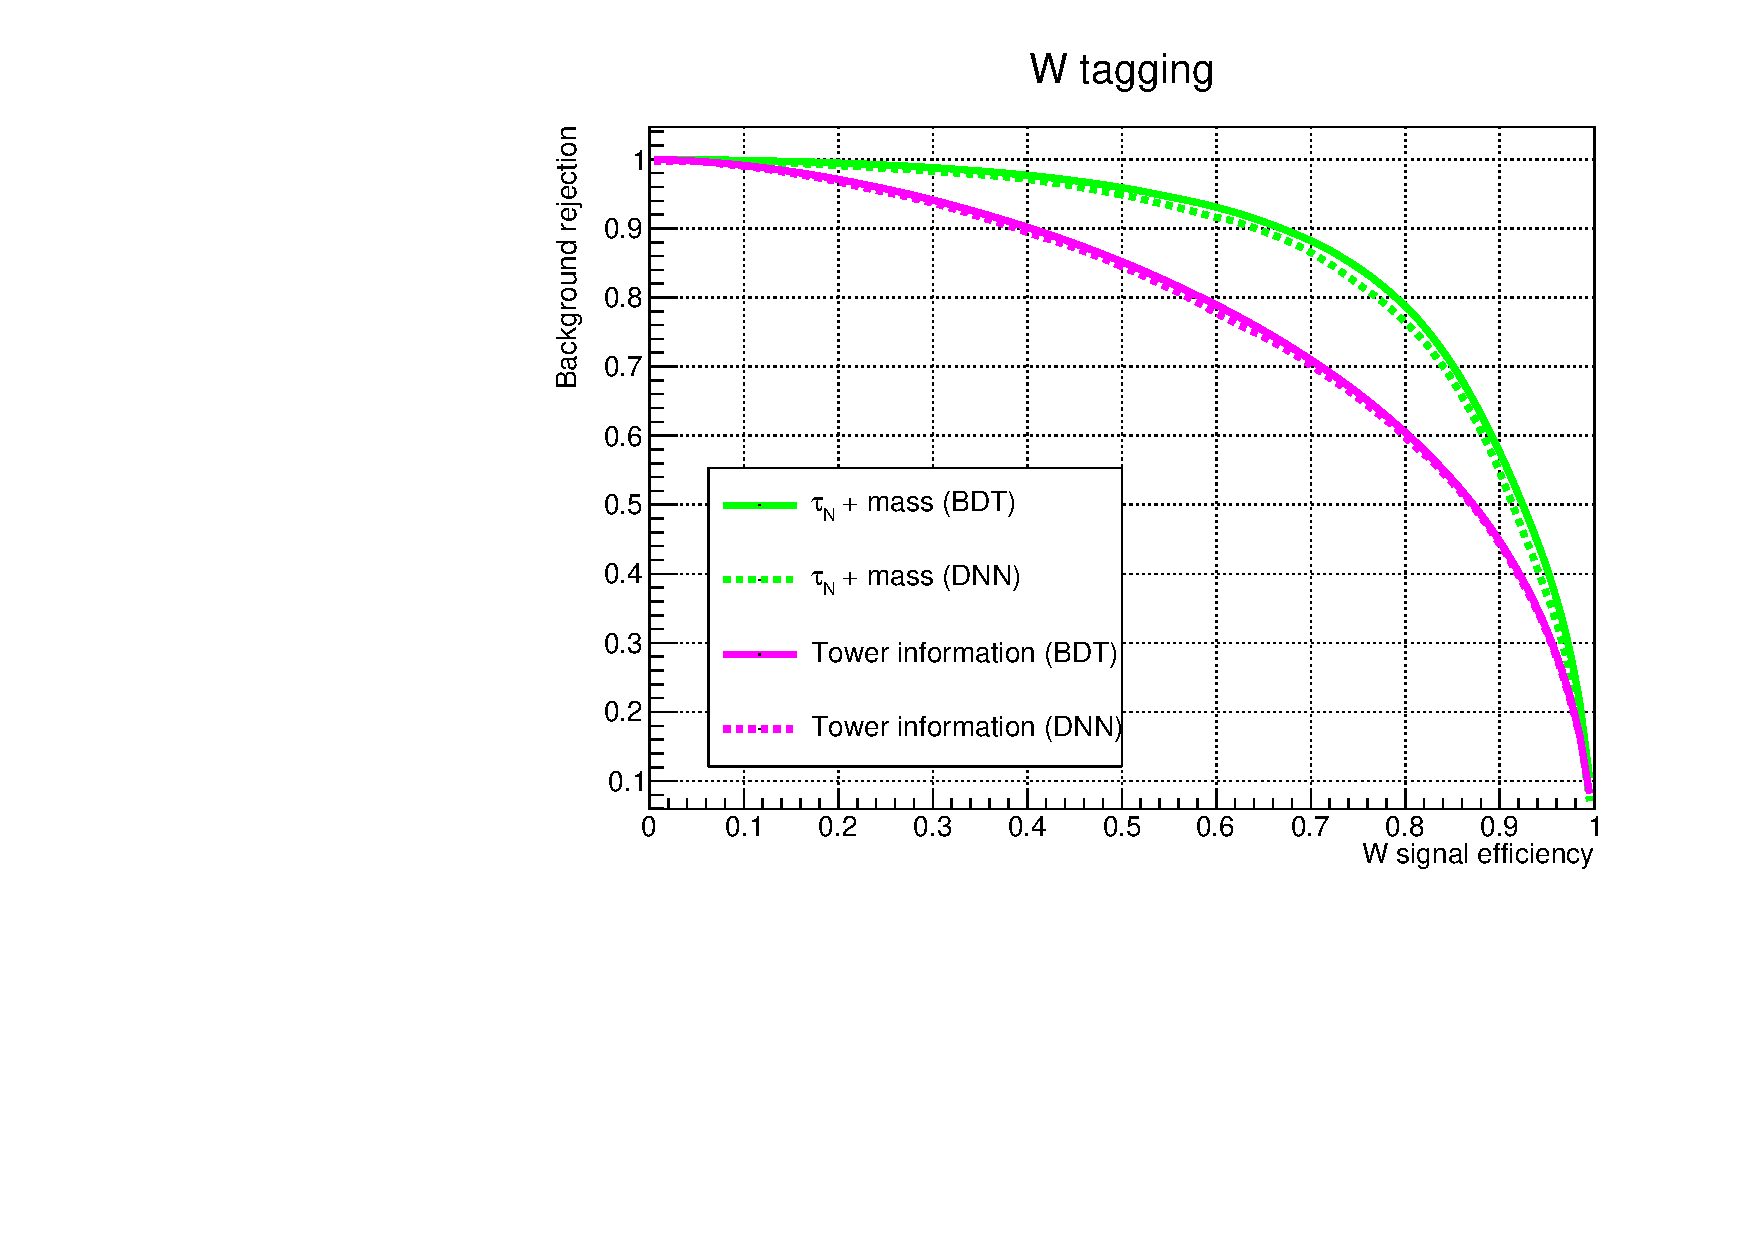
\includegraphics[width=\textwidth]{../Figures/Results/constituents/W_constituents.pdf}
          \caption{}
         \label{fig:W_constituents}
     \end{subfigure}
     \caption{ROC curves for (a) boosted top tagging (b) boosted $W$ tagging using information from the fat jet substructure and from the calorimeter towers as input variables.}
     \label{fig:ROC_constituents}
\end{figure}

The full set of cinematic variables for all towers in each event can not be used due to hardware limitations. Therefore, only the cinematic information of constituents with $E_T$ above the threshold is included. The contribution of the information of towers with lower $E_T$ is expected to be negligible nonetheless. As can be seen from the ROC curves presented above, a far better tagging performance is obtained when the substructure variables are used for the classifier training. This exhibits an advantage of these variables over the ones related to the fat jet constituents: much more information useful for discrimination is contained in a smaller number of variables. This is crucial for machine learning methods in general, where the aim is to have the algorithms learn as much as possible during the training process using a smaller input size, in order to avoid overtraining or running into hardware limitations. 

















% \bibliographystyle{../../PhilReview} %%bib style found in bst folder, in bibtex folder, in texmf folder.
% \nobibliography{Zotero} %%bib database found in bib folder, in bibtex folder
% \nobibliography{../../Thesis_bib}
\biblio

\end{document}
